%%%%%%%%%%%%%%%%%%%%%%%%%%%%%%%%%%%%%%%%%
% Short Sectioned Assignment
% LaTeX Template
% Version 1.0 (5/5/12)
%
% This template has been downloaded from:
% http://www.LaTeXTemplates.com
%
% Original author:
% Frits Wenneker (http://www.howtotex.com)
%
% License:
% CC BY-NC-SA 3.0 (http://creativecommons.org/licenses/by-nc-sa/3.0/)
%
%%%%%%%%%%%%%%%%%%%%%%%%%%%%%%%%%%%%%%%%%

%----------------------------------------------------------------------------------------
%	PACKAGES AND OTHER DOCUMENT CONFIGURATIONS
%----------------------------------------------------------------------------------------

\documentclass[paper=a4, fontsize=11pt]{scrartcl} % A4 paper and 11pt font size

\usepackage[T1]{fontenc} % Use 8-bit encoding that has 256 glyphs
\usepackage{fourier} % Use the Adobe Utopia font for the document - comment this line to return to the LaTeX default
\usepackage[english]{babel} % English language/hyphenation
\usepackage{amsmath,amsfonts,amsthm} % Math packages

\usepackage{lipsum} % Used for inserting dummy 'Lorem ipsum' text into the template

\usepackage{sectsty} % Allows customizing section commands
\allsectionsfont{\centering \normalfont\scshape} % Make all sections centered, the default font and small caps

\usepackage{fancyhdr} % Custom headers and footers
\pagestyle{fancyplain} % Makes all pages in the document conform to the custom headers and footers
\fancyhead{} % No page header - if you want one, create it in the same way as the footers below
\fancyfoot[L]{} % Empty left footer
\fancyfoot[C]{} % Empty center footer
\fancyfoot[R]{\thepage} % Page numbering for right footer
\renewcommand{\headrulewidth}{0pt} % Remove header underlines
\renewcommand{\footrulewidth}{0pt} % Remove footer underlines
\setlength{\headheight}{13.6pt} % Customize the height of the header

\numberwithin{equation}{section} % Number equations within sections (i.e. 1.1, 1.2, 2.1, 2.2 instead of 1, 2, 3, 4)
\numberwithin{figure}{section} % Number figures within sections (i.e. 1.1, 1.2, 2.1, 2.2 instead of 1, 2, 3, 4)
\numberwithin{table}{section} % Number tables within sections (i.e. 1.1, 1.2, 2.1, 2.2 instead of 1, 2, 3, 4)

%\setlength\parindent{5pt} % Removes all indentation from paragraphs - comment this line for an assignment with lots of text

%----------------------------------------------------------------------------------------
%			ADDED PACKAGES, ETC.
%----------------------------------------------------------------------------------------
\usepackage{setspace} % Allows for double spacing, etc.
\usepackage{listings} % for code blocks
\usepackage{color}
 
\definecolor{codegreen}{rgb}{0,0.6,0}
\definecolor{codegray}{rgb}{0.5,0.5,0.5}
\definecolor{codepurple}{rgb}{0.58,0,0.82}
\definecolor{backcolour}{rgb}{0.95,0.95,0.92}
 
\lstdefinestyle{mystyle}{
    backgroundcolor=\color{backcolour},   
    commentstyle=\color{codegreen},
    keywordstyle=\color{magenta},
    numberstyle=\tiny\color{codegray},
    stringstyle=\color{codepurple},
    basicstyle=\footnotesize,
    breakatwhitespace=false,         
    breaklines=true,                 
    captionpos=b,                    
    keepspaces=true,                 
    numbers=left,                    
    numbersep=5pt,                  
    showspaces=false,                
    showstringspaces=false,
    showtabs=false,                  
    tabsize=2
}
 
\lstset{style=mystyle}

\usepackage{hyperref} % links within document
\hypersetup{
    colorlinks=true,
    linkcolor=blue,
    filecolor=magenta,      
    urlcolor=cyan,
}
\usepackage{array}
\newcommand*{\vertbar}{\rule[-1ex]{0.5pt}{2.5ex}}
\newcommand*{\horzbar}{\rule[.5ex]{2.5ex}{0.5pt}}

\usepackage{graphicx}% allows figures
\graphicspath{ {./images/} } 
\usepackage[margin=1in]{geometry}
\usepackage{bm} % allows bold
\usepackage{enumitem}

\DeclareMathOperator{\EX}{\mathbb{E}}% expected value
 
%----------------------------------------------------------------------------------------
%				GLOSSARY
%----------------------------------------------------------------------------------------
% Type these commands at the command line after editing glossary:
% pdflatex summary
% makeglossaries summary
% pdflatex summary

\usepackage{glossaries}
\makeglossaries
\loadglsentries{glossary}
\glsaddall % makes sure all definitions are in glossary even if they aren't mentioned in text

%----------------------------------------------------------------------------------------
%	TITLE SECTION
%----------------------------------------------------------------------------------------

\newcommand{\horrule}[1]{\rule{\linewidth}{#1}} % Create horizontal rule command with 1 argument of height

\title{	
\normalfont \normalsize 
\horrule{0.5pt} \\[0.4cm] % Thin top horizontal rule
\huge Data Science Toolkit \\ % The assignment title
\horrule{2pt} \\[0.5cm] % Thick bottom horizontal rule
}

\author{Matt Goodwin} % Your name

\date{\normalsize\today} % Today's date or a custom date
\onehalfspacing


%----------------------------------------------------------------------------------------
%	BEGIN DOCUMENT
%----------------------------------------------------------------------------------------

\begin{document}

% Print the title
\maketitle 

% Table of Contents
\tableofcontents
\newpage

%----------------------------------------------------------------------------------------
%	SECTION 1
%----------------------------------------------------------------------------------------

\section{Statistical Modeling Overview and Basic Theory}
\subsection{Overview}

When discussing modeling it is important to keep in mind that ``all models are wrong but some are useful'' \footnote{attributed to George Box}. The world is extremely complex and it can be impossible to create a model that perfectly approximates the underlying mechanisms that make our world turn.

There are different approaches to modeling depending on the discipline you come from, but personally I like the idea of the function approximation approach suggested by applied math and statistics. This is the approach that ESL takes. Taking this approach allows us to use probability theory combined with decision theory.

Bishop, from his book \emph{Pattern Recognition and Machine Learning}, has a really nice overview of some of these concepts. The starting point I think for modeling, at least in a supervised setting, starts with the independent variable or covariate $X$ and dependent variable $Y$ (see \hyperref[sec:notation]{notation} section). We want to know:

\begin{enumerate}
\item The nature of the relationship between the variables (inference). 
\item Given an independent variable, determine the dependent variable (prediction).
\end{enumerate}

Bishop mentions that by using probability we can completely summarize the relationship and the uncertainty between the two variables with the joint distribution $P(X,Y)$. We use probability because for many problems we are interested in, we generally cannot come to a completely deterministic relationship between the independent and dependent variables. This is partly because of measurement error, but also because the number of independent variables needed to perfectly determine the dependent variable is potentially infinite. 

For example, imagine we wanted to predict the number of ice cream cones we will sell on a particular day. Some variables such as the time of year or location of the ice cream store may provide us enough information to make a pretty good prediction or to understand the relationship between some of the independent and dependent variables fairly well. But to perfectly predict the number of ice cream cones we would need to know everything from the state of the road conditions, to whether or not a family from out-of-state decided to take a vacation. Since this is impossible, we acknowledge variability and error in our estimates using probability.

I think the key to understanding this is to remember that the moment we use only a subset of all the possible features we would need for a perfectly deterministic relationship, then we must introduce uncertainty. We cannot say for certain that only knowing today is July 1 will lead to high ice-cream sales, but we can say the probability is higher than January 1st. When I have a training sample $(x_1, y_1), (x_2, y_2), ... (x_n, y_n)$,  I treat this as the truth (which it is) but I need to remember that these are draws coming from a distribution. I guess in that sense $P(X,Y)$ is a model itself, something we are forced to use because we don't know all the features needed for a deterministic relationship. 

One side note to make here is, as ESL mentions, sometimes the relationship IS deterministic but the randomness comes from the fact that we have limited data. If we have a different training data set then we get different results but the underlying relationship is still the same since it is deterministic. These types of problems can be handled by similar techniques where the relationship between the variables is probabilistic (see pg 28 of ESL).

Along the above point, it may be tempting to think that the more features the better because we would be getting closer to a deterministic relationship where we could predict perfectly. The issue with this however is related to the problem just mentioned that when we build models we have only a sample from the distribution. We could then start to tune our model to the specific data set but not the true distribution. So I imagine a lot of features would be fine to have, but only if we have more and more data that approximate the true distribution. See the \hyperref[sec:curse]{section} on curse of dimensionality for more discussion along this point.

\subsection{Decision Theory}
As mentioned above, one key area of interest in understanding the relationship between $X$ and $Y$ is inference, or in other words understand what $P(X,Y)$ looks like using information from a sample.  This can give us an understanding of how the variables are related. In many practical applications however, we want to be able to predict $Y$ given $X$. This is where decision theory comes into play. Decision theory is designed to help us make the optimal decision given inputs. Bishop gives a nice overview that I try and summarize in my own words below.

Lets approach this by treating the dependent variable $Y$ as a categorical variable taking on values 0 or 1. For simplicity assume $X$ is a single continuous variable. We then have for $P(X,Y)$ a three-dimensional distribution where $P(Y|X)$ is a probability mass function. When making a decision called the \emph{decision step} we formulate some rule that divides the input space into \emph{decision regions}. If an instance falls into a certain decision region (based on $X$) it is predicted to be a 0 or 1. We want to minimize our mistakes as much as possible so we aren't assigning an instance to 0 when it should really be 1. The probability of a mistake can be written as:

\begin{equation}
P(mistake) = P(X\in R_1, 0) + P(X\in R_0, 1)
\end{equation}
where $R_1$ is the region where an instance is assigned a 1 and $R_0$ is the region where an instance is assigned a 0.

Back to our example. Instead of ice cream sales, treat $Y$ as a categorical variable where 1 is a ``good'' ice cream sales day and 0 is ``bad''.  If $x_1$ = ``July 1st'' is in $R_1$ we decide to assign it a 1, based on our decision rule. However, even though our model $P(X,Y)$ says that the probability of a high-selling day ($Y=1$) is high in this region, there is a still a chance that it is a low-selling day because again, we are using a probability distribution for a model since we don't have all of the features we need for a deterministic model. The probability of it being a low-selling day for all $X$ in $R_1$ is $P(X\in R_1, 0)$, which is a mistake.

 \begin{figure}[t] \label{fig:bishop_optimal_distributions}
\caption{Plot from Bishop showing visually the optimal decision boundary}
\centering
 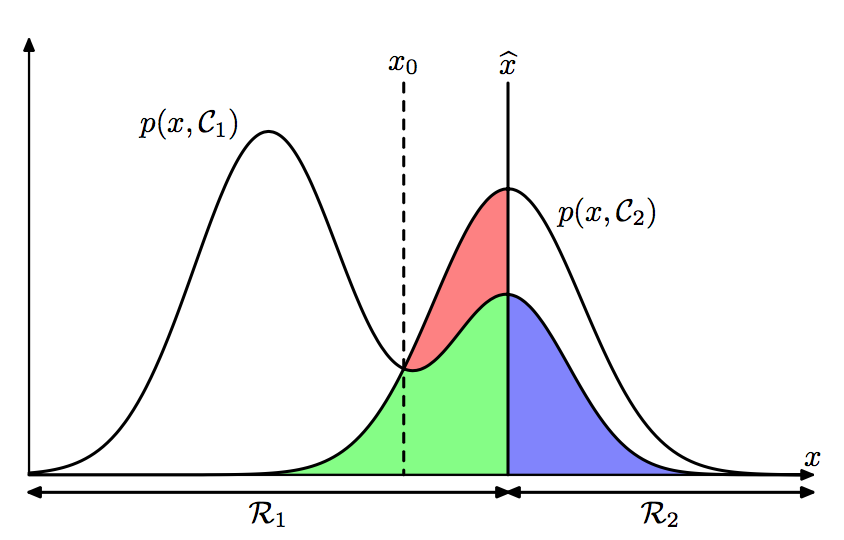
\includegraphics[scale=.7]{bishop_optimal_distributions.png}
 \end{figure}
 
We want to minimize our mistakes as much as possible so we choose regions where $P(X\in R_1, 0) + P(X\in R_0, 1)$ is as small as possible. To me it is easier to see this by thinking of the probability of being correct instead of the probability of being incorrect. This changes the problem from one of minimization to one of maximization. The optimal decision boundary therefore is the location that creates $R_1$ and $R_0$ such that $P(X\in R_1, 1) >  P(X\in R_1, 0)$ everywhere in $R_1$ and $P(X\in R_0, 0) >  P(X\in R_0, 1)$ everywhere in $R_0$. If the decision boundary were shifted either way then we would loose out on area under the distribution of being correct. 

To visualize this better refer to figure \ref{fig:bishop_optimal_distributions} from Bishop which is on pg 40 in his book. If our decision boundary were at $x_0$ then the probability of being correct would be the two humped distribution completely colored in. This is the largest the probability of being correct can be. If we went with $\hat{x}$ however, then we loose out on the red region for being correct, which is suboptimal. (I like to think of a three dimensional distribution here whereas Bishop has an image with two different distributions which would need to be normalized appropriately but the concept is the same).

 We can use the product rule to write:
 
 \begin{equation}
 \begin{split}
 P(X\in R_1, 1) >  P(X\in R_1, 0)  & \implies  P(1|X\in R_1) P(X \in R_1) > P(0|X\in R_1) P(X \in R_1) \\
 & \implies  P(1|X\in R_1) > P(0|X\in R_1) 
 \end{split}
 \end{equation}
 So the maximization problem is equivalent to choosing the higher conditional probability for each region. This rule is known as the \emph{Bayes classifier} and the error rate of the Bayes classifier is known as the \emph{Bayes rate}. The Bayes classifier is used as a benchmark in classification as it is the optimal solution to classification if the probability distributions are known.
 
\subsection{Expected Loss Function}
Embedded in the above discussion describing how to find the optimal decision rule is a concept called the \emph{loss function}. This is a function that takes as input the true class and predicted class (resulting from the chosen decision rule) and outputs a value encoding the error of the prediction. We can use this formulation to find the optimal decision rule by minimizing the function with respect to the decision rule.

In the above examples we assume that the loss function is outputting a 0 for each class predicted correctly and a 1 for each class predicted incorrectly, so in other words all classes are weighted the same in terms of misclassification (this is also known as the 0-1 loss function). In some applications however, such as medical diagnosis, we want to weight some classes higher than others when calculating misclassification. For example, when diagnosing cancer it is much better to predict someone who is healthy as having cancer than the other way around.

For classification we can think of this function as a matrix known as the \emph{loss matrix}, but in general we can think of it as taking in two variables - the true class and the predicted class:

\begin{equation}
L(G, \hat{G}(X)).
\end{equation}
where $G$ is the true class and $\hat{G}(X)$ is the predicted class - $X$ representing the independent variables.

As Bishop points out, one issue with using this measure however is that we don't know the true class $G$. We can choose some decision rule to get us $\hat{G}$, but since we are dealing with probability distributions we won't know for sure whether the true class is a high-sales ice cream day or a low-sales ice cream day for example. Instead of finding $\hat{G}$ that minimizes the loss function, we can instead minimize the expectation of the loss function or in other words minimize the average loss function weighted by the probabilities for $G$ and $X$.

\begin{equation}
\begin{split}
E[L(G, \hat{G}(X))] & = \iint_{G, X} {L(G, \hat{G}(X)) P(G, X) dG dX} \\
& = \int_{X} \sum_{k=1}^{K} {L(G_k, \hat{G}(X)) P(G_k|X) P(X) dX} \\
&= E_{X} \sum_{k=1}^{K} {L(G_k, \hat{G}(X)) P(G_k|X)}
\end{split}
\end{equation}
where $k=1,...K$ are the different classes, in our example either 0 or 1. We want to find a classifier $\hat{G}(X)$ such that the expected loss is minimal. As ESL illustrates, to do this we can minimize the inner quantity pointwise since this corresponds to the minimum of the entire quantity (the minimum of an average is the minimum of the separate quantities in the average). This leads us to write:

\begin{equation}
\hat{G(x)} = \text{argmin}_{g \in G} \sum_{k=1}^{K} {L(G_k, g) P(G_k|X)}
\end{equation}
If we are using the 0-1 loss function then we can simplify this to:

\begin{equation}
\hat{G(x)} = \text{argmin}_{g \in G} \left[1 - P(g|X=x) \right].
\end{equation}
This took some thought for me to understand why we could simplify down to this. I think the best way to see it is to remember that this is a function of $g$. If we have $K=3$ for example then we can write out for each possible value of $G_k$:

\begin{equation}
\begin{split}
g=G_1 & \implies P(G_2|X=x) + P(G_3|X=x) \implies 1-P(G_1|X=x)\\
g=G_2 & \implies P(G_1|X=x) + P(G_3|X=x) \implies 1-P(G_2|X=x)\\
g=G_3 & \implies P(G_1|X=x) + P(G_2|X=x) \implies 1-P(G_3|X=x)\\
\end{split}
\end{equation}
since our loss function is 0 when it is a true classification and 1 when it is a misclassification. Since we are minimizing, the best choice for $g$ is the one where $P(g|X=x)$ is the largest (for each $x$) which corresponds to the Bayes classifier. Thus, we have proven that under the 0-1 loss function, the optimal decision is the Bayes classifier as we found in our previous discussion. Note that this is optimal when we know the distribution which most times we don't. The point to make here is that in the presence of uncertainty, the Bayes classifier is really the best we can do under the 0-1 loss function.

The above discussion is more theoretical in nature than practical. In reality we will not know what the true distribution looks like, and instead only have a sample to work with. Therefore to make this minimization problem more practical we need to include the random variable that represents the sampling process. To see this better we should then write the expected loss in the form of two expectations. The first is known as the \emph{test error}, the \emph{generalization error}, or \emph{prediction error}, all according to ESLII:

\begin{equation}
E[L(G, \hat{G}(X))|T]
\end{equation}
where the variable $T$ represents the training set.  Optimizing this expectation now should yield a different answer than before because of the dependence on $T$. We can also think of this quantity as the expected loss given training set $T$.

If we take an expectation over all training sets and everything that is random then we have the original expected loss talked about earlier:

\begin{equation}
\begin{split}
E_{T}[E[L(G, \hat{G(X)})|T]] &= E_{T}[E_{G,X}[L(G, \hat{G(X)})|T]] \\
&= E_{T}\left[\iint_{G, X} {L(G, \hat{G}(X)) P(G,X|T) dG dX}\right]\\
&= \iiint_{G, X, T} {L(G, \hat{G}(X)) P(G,X|T) P(T) dG dX dT} \\
&= \iiint_{G, X, T} {L(G, \hat{G}(X)) P(G,X,T) dG dX dT}\\
&= E_{G,X,T}[L(G, \hat{G}(X))]\\
&= E[L(G, \hat{G}(X))]
\end{split}
\end{equation}
ELSII calls this the \emph{expected test error} or \emph{expected prediction error}. This measures how well our average model generalizes to the entire population, where average model is referring to the average model over all training sets $T$. 

Really our goal at this point according to ESLII, would be to find (or approximate with a sample) the prediction error for a given training set $T$. This is the goal because we are only given one training set and we want to know what the generalization error is over the entire distribution of $G, X$ for the model derived from that particular training set. It appears that this is harder to do in practice and most methods actually estimate the \emph{expected} prediction error better. Therefore we will focus on estimating the expected prediction error. See ESLII pg. 220 for more discussion.

The discussion of the loss functions above uses random variables and expectations and is referring to when we know the distributions involved. In practice however, we are only given a sample from that distribution and so when finding a model we use whats known as the \emph{cost function} which adds up the loss function for each data point being used:

\begin{equation}
J(\theta) = \sum_{i=1}^{N}{L(g_i, \hat{G_\theta}(x_i))}
\end{equation}



%\noindent TODO: Show graphs of general loss functions - see Stanford machine learning cheat sheet \newline
%TODO: I think the expected loss is also known as the Risk function \newline
%TODO: Show the regression loss function formulation. Note that the conditional mean is the optimal decision under the least squares loss just like the Bayes classifier is under the 0-1 loss. These loss functions are nice theoretically but may not be realistic in practice \newline
%TODO: Explore the idea that the conditional mean is optimal IF we know the distribution just like the Bayes Classifier is optimal IF we know the distribution. \newline
%TODO: Why is the predicted error what we want? How does the training vs. cross validation vs. testing error fit in here?

\subsection{Bias-Variance Tradeoff}

The bias-variance tradeoff refers to two sources of error when evaluating models - the bias and the variance. There is also a third source of error which we call the ``irreducible error''. 

As explained in \href{https://towardsdatascience.com/mse-and-bias-variance-decomposition-77449dd2ff55}{this} article, there is a slight confusion in data science between decomposing the error for an \gls{estimator}, and decomposing the error for a model or a predictor. The decomposition is really about the same but there are some key insights to be aware of. The decomposition below is for a predictor. The decomposition for an estimator can be found in various books and other resources such as Casella/Berger. 

First of all the bias of a model is defined as:

\begin{equation}
\text{Bias}\left(\hat{f}(X)\right) = E \left[\hat{f}(X) - f(X)\right]
\end{equation}
and variance of a model is:

\begin{equation}
\text{Var}\left(\hat{f}(X)\right) = E \left[\hat{f}(X)^2\right] - E \left[\hat{f}(X)\right]^2. 
\end{equation}
Knowing these definitions we can then take the expected loss function and perform the following decomposition (assuming squared error loss):

\begin{equation}
\begin{split}
E[L(Y, \hat{f}(X))] & = E_{T}[E_{Y,X}[L(Y, \hat{f(X)})|T]] \\
&= E_{X,Y|T}[E_{T}[L(Y, \hat{f(X)})]]  \quad \text{(Drop $|T$ at this point since inner expectation is over $T$)}\\
&= E_{X,Y}[E_{T}[(Y - \hat{f}(X))^2]] \\
&= E_{X,Y}[E_{T}[(Y^2 - 2Y\hat{f}(X) + \hat{f}(X)^2)]] \\
&= E_{X,Y}[E_{T}[Y^2] - E_{T}[2Y\hat{f}(X)] + E_{T}[\hat{f}(X)^2] + E_{T}[\hat{f}(X)]^2 - E_{T}[\hat{f}(X)]^2]\\
&= E_{X,Y}[Y^2 -  2YE_{T}[\hat{f}(X)] + E_{T}[\hat{f}(X)^2] + \text{Var}_{T}(\hat{f}(X))]\\
&=E_{X,Y}[(Y - E_{T}[\hat{f}(X)])^2 + \text{Var}_{T}(\hat{f}(X))] \\
&= E_{X,Y}[\text{Bias}_{T}(\hat{f}(X))^2 + \text{Var}_{T}(\hat{f}(X))] 
\end{split}
\end{equation}
This shows that for the squared error loss we can decompose the expected loss function into a bias term and a variance term. There is typically an irreducible error term in most decompositions but those decompositions make additional assumptions (such as constant variance) and I wanted to stay more general. In reality the irreducible error term is rolled up in the expectation over $X,Y$. One another note to make here is that I think we can drop the condition on $T$ in the derivation since the only quantity that depends on $T$ is the model $\hat{f}(x)$ and since the model is wrapped up in an expectation over $T$ then we don't need to worry about the conditional.

What this decomposition reveals are different sources for error. The variance term reveals how much a model varies over training sets. The bias term reveals how far off our model is averaged over all training sets. Different models perform differently in regards to these two terms. Linear regression for example has high bias (meaning if we average over all training sets, the model is relatively wrong), but low variance (the model won't change drastically with a new training dataset). Decision trees are the opposite - they have low bias (over all training sets the average tree is relatively not too far off the truth), but high variance (decision trees can look completely different depending on the given training dataset).

It appears that ensembles can decrease both sources of error by averaging low bias models. When we take an average the variance decreases (see discussion on Bagging and Random Forest).

One issue that isn't as satisfying to me here is that this neat decomposition appears to be for squared-error loss only. Most textbooks leave the bias-variance decomposition discussion at this point. What bugs me is there is really no discussion about this decomposition for a \emph{general} loss function. One paper I found that addresses this issue (sort-of) is found \href{https://homes.cs.washington.edu/~pedrod/bvd.pdf}{here} by Pedro Dominguez. I'd like to explore this a little more. Also see \href{https://github.com/rasbt/mlxtend/blob/master/docs/sources/user_guide/evaluate/bias_variance_decomp.ipynb?utm_campaign=Data_Elixir&utm_source=Data_Elixir_210}{here} for a python package that gives you the decomposition and refers to the Dominguez paper.




\subsection{Generative vs. Discriminative Models}

The previous discussions about probability distributions that explain the relationship between dependent and independent variables sets us up nicely for understanding what generative vs. discriminative models are. Bishop does a good job explaining the difference. \textbf{Generative models} are models that attempt to find or approximate the original distribution $P(X,Y)$. They are called generative because once we've found a generative model we can \emph{generate} synthetic data from the model, inputs AND outputs. We can also use generative models to make predictions by using Bayes rule to find the posterior distribution $P(Y|X)$ and then use decision theory to make the prediction (essentially assign the instance to the class with the highest probability distribution, if we are using a traditional loss function). \textbf{Discriminative models} attempt to model the posterior density $P(Y|X)$ directly and then use decision theory to make predictions using that posterior density. 

Both of these approaches first do whats called the \emph{inference stage} (finding the distribution) and then use the posterior probabilities in the \emph{decision stage}. A third option exists where we directly find a function $f(X)$ that maps inputs to outputs. The function $f(X)$ is known as a \emph{discriminant function}.

There are pros and cons to each approach as Bishop mentions which I summarize here:
\break

\noindent \underline{\textbf{Generative model pros}}:
\begin{itemize}
\item Allows us to find the marginal density $P(X)$ which tells us the likelihood of given inputs and helps us identify inputs that may not be common and therefore less accurate. This is a form of outlier detection.
\item Allows us to generate synthetic data
%\item TODO: Read Andrew Ngs' and Michael Jordan's paper on the comparison between generative vs. discriminative
\end{itemize}

\noindent \underline{\textbf{Generative model cons}}:
\begin{itemize}
\item Could be considered a waste of effort if only goal is prediction. 
\item Since we are attempting to find the entire density $P(X,Y)$ we may need more data in order to find accurate posterior distributions.
\end{itemize}

\noindent \underline{\textbf{Discriminative model pros}}:
\begin{itemize}
\item Once we've found this model and our loss function changes, then we only need to change the loss function - we don't need to retrain the entire model compared to the discriminate function approach.
\item Reject option - Bishop likes this concept where we can determine areas we aren't as confident the model can do a good job with and instead ask a human to make the classification.
\item We can deal better with class imbalance - TODO: Bishop has a good synopsis that I might write in later
\item Combine models - TODO: Gives an example of the naive Bayes model
\end{itemize}

%TODO: I think I've made a connection here between the discriminative model and discriminative function. For least squares the optimal decision is the condition mean and that is what f(x) is below.

The discriminative model $P(Y|X)$ allows us, as Bishop says,  to completely summarize the way $Y$ depends on $X$. When we use another model like the additive error model, we make a further assumption that the errors are independent of $X$ and that they have a constant variance. So the additive error model puts further constraints on the discriminative model. We can still think of the additive error model as some conditional distribution, but a distribution that is simplified.

We can also go the other direction by thinking of the discriminative model $P(Y|X)$ as the equation $y_i = f(x_i) + \epsilon_i$ but not putting constraints of any kind on $\epsilon_i$. The idea is that there is some "true function" out there and then there are some errors off of that true function that gives us our dependent variable.

% TODO: In either case the next step is to then think of other modeling assumption for $f(x_i)$ such as the linear model.


\subsection{Curse of Dimensionality} \label{sec:curse}

The \emph{curse of dimensionality}  \footnote{attributed to Richard Belllman} refers to the problem that models face in many dimensions. As both ESL and Bishop describe, our intuition break down in many dimensions. For example, Bishop gives the example of points in a unit sphere. In general the volume of a hypersphere can be written as:

\begin{equation}
V_n(R) = \frac{\pi^{\frac{n}{2}}}{\Gamma(\frac{n}{2} + 1)}R^n.
\end{equation}
where $R$ is radius, $n$ is the number of dimensions and $\Gamma$ is the \gls{gamma} function. So for example if we are in two dimensions $(n=2)$ we would get:

\begin{equation}
\frac{\pi}{\Gamma(2)}R^2 = \pi R^2.
\end{equation}
What is interesting is if we consider a hyper sphere in $D$ dimensions and then an inner hyper sphere of radius $\epsilon$ contained within the larger sphere. If we write out the volume between these two spheres, hold radius to 1, and consider this quantity as a proportion to the larger outer sphere we get:

\begin{equation}
\frac{\frac{\pi^{\frac{D}{2}}}{\Gamma(\frac{D}{2} + 1)} - \frac{\pi^{\frac{D}{2}}}{\Gamma(\frac{D}{2} + 1)} (1-\epsilon)^{D}}{\frac{\pi^{\frac{D}{2}}}{\Gamma(\frac{D}{2} + 1)}}
\end{equation}
Simplifying we are left with:
\begin{equation}
1 - (1-\epsilon)^D.
\end{equation}

From this equation we can see that as we increase the dimension $D$, the quantity gets closer and closer to 1. Since the quantity is a proportion over the outer sphere this implies that most of the volume is in between the inner sphere and the outer sphere as the dimension increases. This is even true when the inner sphere is close to the same size as the outer sphere (when 1-$\epsilon$ is really small).

A better example roughly given by Bishop illustrates the issue when applied to modeling. Consider a naive model where for each new data point we assign a predicted label according to a majority rule within a uniform neighborhood (similar to nearest neighbors but splitting the space up into uniform cubes instead of a neighborhood around each data point). In one dimension say we look at the range between 0 and 4 and split the space up into 4 intervals of 1 unit each. If we are given a new point, 1.5 for example, then we assign that data point the majority label of all other points in the interval 1 to 2. 

Say however, that we add a second dimension with the same range. The number of unit squares will now be 16. If we go to three dimensions we now have 64 squares, four dimensions 256, etc. This is an issue because in order to determine what each point should be in a given unit cube, we need to make sure we have data in each cube, implying that we need an exponentially increasing amount of data as we increase our dimensions. More specifically in one dimension we would need at least 4 data points to have a data point in each interval, but in four dimensions we would need at least 256 data points (however, in both scenarios there is no guarantee that we get a data point in each interval or cube, this just illustrates a general rule).

% TODO: I don't understand this local part very well
So what to do if we have limited data and many dimensions? There are a couple of ideas from Bishop to keep in mind that give us hope. The first idea is that in practice data tends to be more concentrated. This implies that the true dimensionality is potentially much lower. The other idea that Bishop mentions is that "real data will exhibit some smoothness properties" locally (see pg. 37). This I think implies that we can use models that rely on these assumptions. This last point is a little fuzzy to me still but I think ESL (on pg 32-33) sheds a little light by talking about the \emph{complexity} of a model, in particular restraining the complexity of the model. As ESL mentions "this usually means some kind of regular behavior in small neighborhoods of the input space". Instead of using a nearest neighbor type approach for example, we can assume the data is linear in these local neighborhoods (which is a constraint on complexity) and use linear regression. The central tradeoff is that for models that do really well locally (nearest neighbors) face the curse of dimensionality and models that overcome the curse of dimensionality may not do well locally.

In summary, the curse of dimensionality is an important concept to keep in mind because it invalidates or severely handicaps naive models such as nearest neighbors in high dimensions and has forced the field of statistical modeling to develop more clever models. Many of these models include various assumptions (pg. 27 of ESL) to get at the true nature of the data, such as linear regression. When these assumptions are correct then the models have a chance at performing well and we have avoided the "exponential growth in complexity of functions" (ESL).


\subsection{No Free Lunch Theorem}

Bishop has a great summary of this concept from a \href{https://www.microsoft.com/en-us/research/blog/machine-learning-and-the-learning-machine-with-dr-christopher-bishop/}{podcast} with Microsoft Research. To paraphrase, the No Free Lunch Theorem implies that all machine learning algorithms perform equally, averaging across all possible problems. In other words as Bishop says "there cannot be a single universal machine learning algorithm that will solve all problems" (see podcast transcript). 

The caution here however is that this theorem is more of an abstract concept and really there may be algorithms that perform consistently well on the problems we care about or that we see in the real world (think deep learning for example). The larger point to take-away as Bishop mentions however, is that there are really two parts to a problem: the data and the assumptions (or in other words priors, constraints, etc.). Both are important  and he makes the case for treating assumptions as "first-class citizens", not just the data. This makes a lot of sense to me because if our data is truly linear then a linear model would potentially do much better than a decision tree for example.


\newpage



\section{Assessment of Models}
\subsection{Classification Metrics}
\subsubsection{Confusion Matrix}
Perhaps the place to start when evaluating classification models is the confusion matrix. Figure \ref{fig:confusion} shows an excellent figure from Wikipedia displaying what this matrix looks like.

 \begin{figure}[h] \label{fig:confusion}
\caption{Plot from Wiki showing confusion matrix}
\centering
 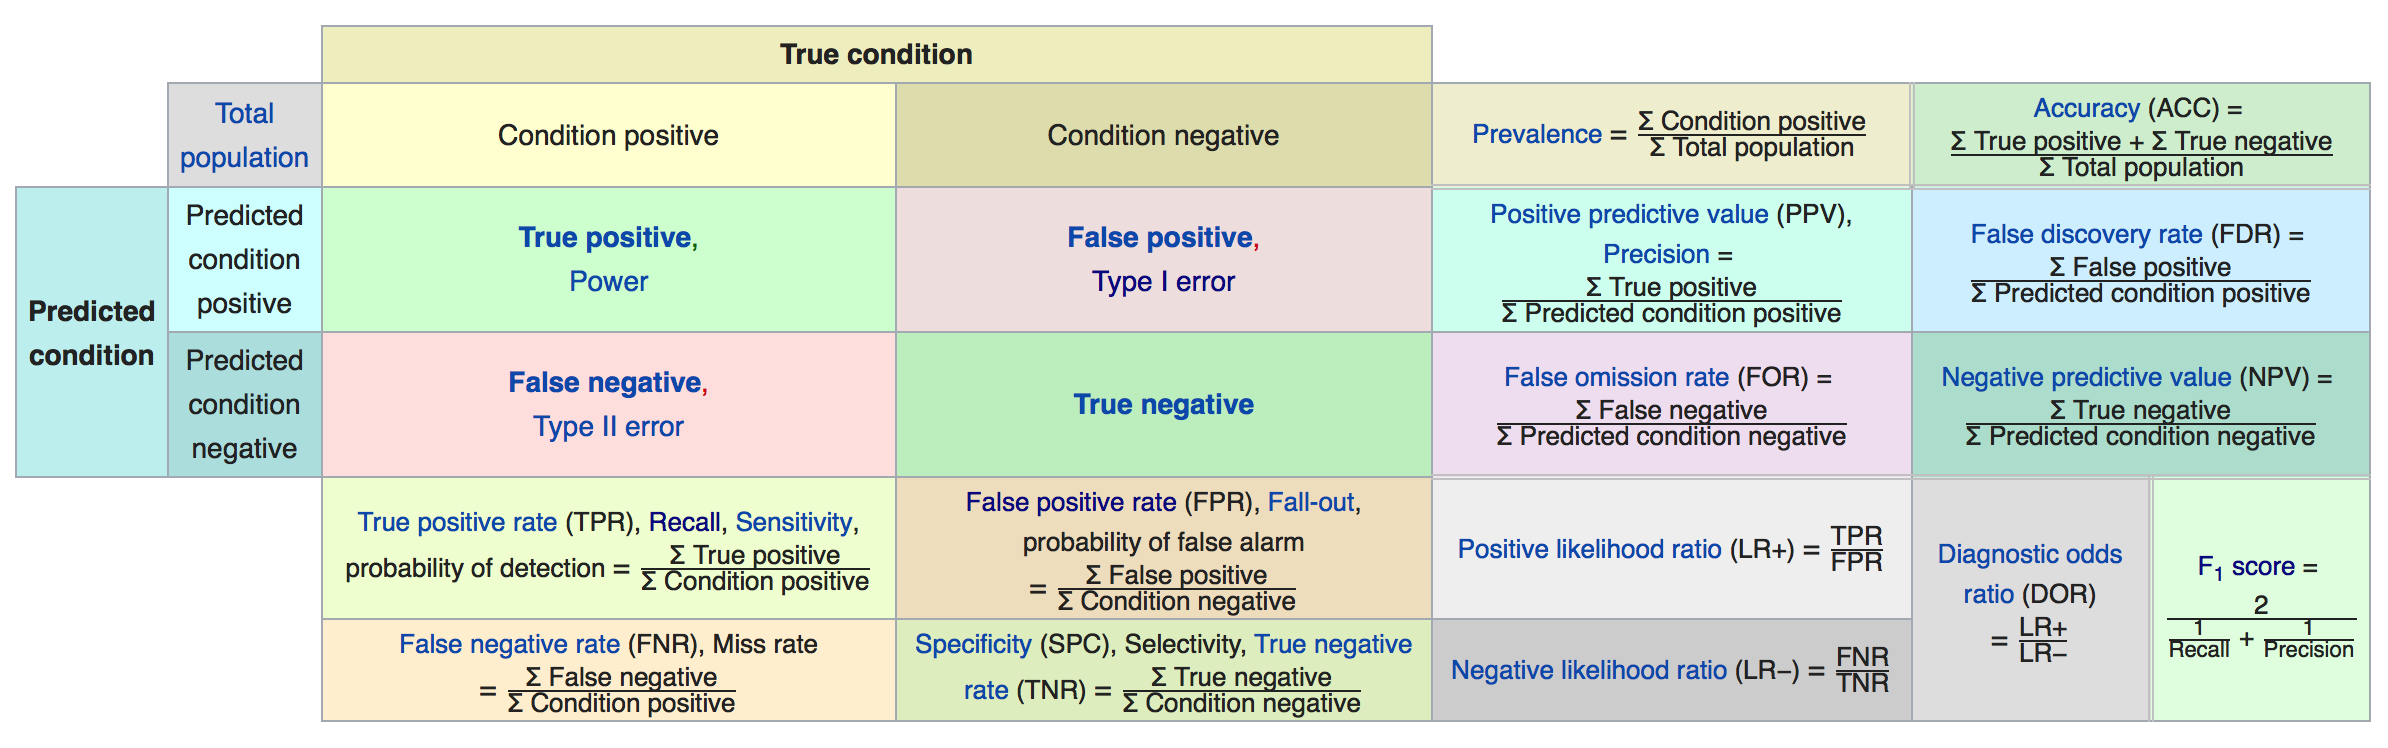
\includegraphics[scale=.4]{confusion_matrix.png}
 \end{figure}
 
 The columns represent the true class (positive or negative) and the rows represent the predicted class (positive or negative). The cross-intersection of these predictions and truth create four areas: \emph{true positives} (number of instances that are predicted positive that actually are positive), \emph{false positives} (number of instances that are predicted positive that are actually negative), \emph{false negatives} (number of instances that are predicted negative that are actually positive) and \emph{true negatives} (number of instances that are predicted negative that actually are negative).
 
 In the Wiki figure there are three other terms in the 2x2 confusion matrix namely power, Type 1 error, and Type 2 error. TODO
 
 

\section{Generalized Linear Models}

There are three main components that make up the Generalized Linear Model (GLM):

\begin{enumerate}
\item Random component - assume the response variable comes from a probability distribution
\begin{equation}
Y_i \sim f(\mu_i)
\end{equation}
where $\mu_i = E(Y_i)$ and $f$ is a probability distribution.
\item Link component - connects the random component to the systematic component
\begin{equation}
g(\mu_i)=\eta_i
\end{equation}
\item Systematic component - this is the linear part
\begin{equation}
\eta_i = x_i^\prime \beta
\end{equation}

\end{enumerate}


\subsubsection{Logistic Regression}

Using the component concepts outlined above, for logistic regression we have:

\begin{enumerate}
\item Random component: $Y_i \sim f(\pi_i)$ where $f$ is the Bernoulli distribution (since $Y$ will be a binary variable when using logistic regression). $E(Y_i) = \pi_i $ which is the probability that $Y_i$ is 1.
\item Link component: this is the logit function which is defined as:
\begin{equation}
\text{logit}(\pi_i) = \log \left(\frac{\pi_i}{1-\pi_i} \right) = \eta_i
\end{equation}
\item Systematic component: tying this all together we have:
\begin{equation}
\log \left(\frac{\pi_i}{1-\pi_i}\right) = x_i^\prime \beta
\end{equation}
\end{enumerate}

Assumptions:
\begin{enumerate}
\item Linearity in log-odds
\item Independence of $Y_i|x_i$ and $Y_j|x_j$
\item Bernoulli response variable
\end{enumerate}

For interpretation we can say that with a one unit increase in $X_1$ for example, then the log odds of a success goes up by $\beta_1$. We can also use the multiplicative odds where a one unit increase in $X_1$ leads to a $e^{\beta_1}$ multiplicative change in odds on average.

The probability can be calculated by:
\begin{equation}
\begin{split}
\log \left(\frac{\pi_i}{1-\pi_1} \right) & = \beta_0 + x_i \beta_1 \\
\frac{\pi_i}{1-\pi_i} &= e^{\beta_0 + x_i \beta_1} \\
\pi_i &= e^{\beta_0 + x_i \beta_1} - e^{\beta_0 + x_i \beta_1} \pi_i \\
\pi_i &= \frac{e^{\beta_0 + x_i \beta_1}}{1+e^{\beta_0 + x_i \beta_1}}
\end{split}
\end{equation}


\section{Bayesian Statistics}
\subsection{Bayesian Hierarchical Models}

The majority of this section comes from Bayesian Data Analysis (BDA) by Gelman et. al.

The need for hierarchical models arise when we have data that are dependent on parameters, which in turn are related to each other. The example that BDA gives is of the study of cardiac treatment effectiveness. It is reasonable to assume that the data $y_{ij}$ collected over different hospitals come from different parameters, with a parameter for each hospital. We can then treat these parameters as coming from a higher distribution, and then estimate the parameters of the higher distribution based on the data. This allows us to control for the group level effect and helps us fit a better model.

 

\section{Ensemble}
\subsection{Bagging}

Bagging (bootstrap aggregating) is based on the concept that the variance of averaged random variables is less than the variance of the random variables individually. To see this say we have a random sample $X_1,..., X_N$ where the mean of $X_i$ is $\mu$ and the variance is $\sigma^2$ . The expected value of the average of this random sample is $\frac{1}{N}\sum_{i=1}^N{E[X_i]}$ and the variance can be decomposed as:

\begin{equation}
\begin{split}
Var \left(\frac{1}{N}\sum_{i=1}^N{X_i} \right) &=  E\left[ \left(\frac{1}{N}\sum_{i=1}^N{X_i}\right)^2 \right] - E\left[\frac{1}{N}\sum_{i=1}^N{X_i}\right]^2 \\
&= E\left[ \left(\frac{1}{N}\right)^2 \left(\sum_{i=1}^N{X_i}\right)^2 \right] - \left(\frac{1}{N} \right)^2 E\left[\sum_{i=1}^N{X_i}\right]^2 \\
&= \left(\frac{1}{N} \right)^2 \left( E\left[\left(\sum_{i=1}^N{X_i}\right)^2 \right] - E\left[\sum_{i=1}^N{X_i}\right]^2    \right) \\
&= \left(\frac{1}{N} \right)^2 Var\left(\sum_{i=1}^N{X_i}\right)\\
&= \left(\frac{1}{N} \right)^2 N \sigma^2\\
&= \frac{\sigma^2}{N}
\end{split}
\end{equation}
The second to last step is possible because the $X_i$ are independent and the variance of a sum of independent variables is the sum of the variances. Since $X_i$ are identically distributed then the variance will be $\sigma^2$ for all $X_i$.

This same idea applies to predictors or models. To apply this concept to models, $B$ bootstrapped samples are derived and a model $\hat{f}^b(x)$ is built on each sample. These samples are then averaged together:

\begin{equation}
\hat{f}_{bag}(x) = \frac{1}{B} \sum_{b=1}^B{\hat{f}^b(x)}.
\end{equation}

TODO: Expound on bagging a little more especially the connection to a posterior Bayes mean, squared error vs. 0-1, and the error breakdown between bagging vs. single model.

TODO: The method of bagging mentioned previously is an attempt to reduce the variance of models by averaging them together. This seems to work particularly well for noisy, high-variance models such as trees. When we average these trees together the bias does not decrease (related to the idea that the expected value of a random variable is the same as the expected value of the average of i.d. random variables), but the variance does decrease. The amount it decreases depends on whether or not the random variables are i.i.d. or i.d. If i.i.d then variance decreases by a factor of $N$

\subsection{Random Forrest}

Bagging averages models together to reduce error, in particular the variance component to the error. As mentioned, this is analogous to averaging i.i.d. random variables together with variance $\sigma^2$ leading to an overall variance of $\frac{\sigma^2}{B}$ where $B$ are the number of random variables in the average. 

The issue with this approach is when the models (or random variables in our analogy) are correlated. This is the case when using decision trees for example. If use our random variable analogy then 



\subsection{Bumping}
This is where we train models on various bootstrapped samples and choose the best bootstrapped sample and the model on that sample. Essentially we are expanding the space of possible models.

\subsection{Boosting}

The concept of boosting has lead to some of the most powerful algorithms in machine learning. Boosting falls under a general class of algorithms known as ensembles (bagging would be another example of ensemble algorithms where we run separate models and then aggregate at the end by averaging). The general concept of boosting is that we use a \emph{weak learner} (a model that does only slightly better than random guessing) to model the original data, calculate the errors, run a new weak learner model on the errors, combine the results with the first weak learner, and repeat until some stopping criteria (that avoids overfitting). Thus boosting algorithms stack multiple learners on top of each other instead of modeling separately and then combining in some way at the end like bagging.

At its heart boosting is really a simple basis function expansion or an additive model. This type of model attempts to approximate a function by treating it as a linear combination of other functions, usually more simple functions:

\begin{equation} \label{eq:basis_optimization}
f(x) = \sum^{M}_{m=1} {\beta_m b(x; \gamma_m)}
\end{equation}
where $\beta_m$ are the basis function coefficients and $b(x; \gamma_m)$ are the basis functions with parameters $\gamma_m$. 
The ideal way of fitting this model would be to minimize some loss function by finding the optimal parameters $\gamma_m$ and coefficients $\beta_m$ (both for all $m$) all at once, but in practice this can be computationally intensive. 

An alternative to this approach which approximates the optimal solution to \ref{eq:basis_optimization} is \emph{forward stagewise additive modeling}. Instead of optimizing over all basis functions at once we instead optimize over one basis function at a time while keeping all previously found basis functions fixed. To be more clear we first fit a weak learner $f_0(x)$ to the data and then in a loop we find models for $m=1$ to $M$ minimizing the cost function over the training data:

\begin{equation}
(\beta_m, \gamma_m) = \text{arg min}_{\beta, \gamma} \sum_{i=1}^{N}{L(y_i, f_{m-1}(x_i) + \beta b(x_i;\gamma))}
\end{equation}

\begin{equation}
f_m(x) = f_{m-1}(x) + \beta_m b(x;\gamma_m)
\end{equation}
This last equation is the recursive relationship that is often written out to describe boosting but more generally with different notation might be written out as:

\begin{equation} \label{eq:recursive}
F_m(x) = F_{m-1}(x) + f_m(x)
\end{equation}

Any loss function can be used, but its interesting to look at the scenario when the loss function is the squared error loss. In this case we would have:

\begin{equation}
\begin{split}
(\beta_m, \gamma_m)  & = \text{arg min}_{\beta, \gamma} \sum_{i=1}^{N}{L(y_i, f_{m-1}(x_i) + \beta b(x_i;\gamma))}\\
&= \text{arg min}_{\beta, \gamma} \sum_{i=1}^{N}{(y_i - f_{m-1}(x_i) - \beta b(x_i;\gamma))^2}\\
&= \text{arg min}_{\beta, \gamma} \sum_{i=1}^{N}{(r_{im} - \beta b(x_i;\gamma))^2}
\end{split}
\end{equation}
where $r_{im}$ is the residual between the previous model's prediction and the observed target value $y_i$. This implies that when using the squared loss function we are training the $m^{th}$ model on the error of the previous model, which in multiple dimensions is a vector giving us direction and magnitude (this is key when thinking of how this relates to the gradient). The resulting $m^{th}$ model will then be an approximation (not perfect, no models ever are) to the error which is then added to the $(m-1)^{th}$ model to help correct that model. From this perspective we can think of each subsequent model as attempting to approximate the error of the previous model and account for that error in the overall model.

We can use different loss functions that lead to different insights. For example, if we use the absolute value error loss we will end up training our weak learners on the $sign$ function. If we use the exponential loss function then we get Adaboost which is discussed in section \ref{section:ada}.

\subsubsection{Gradient Boosting}

The discussion in the previous discussion is fairly straightforward and intuitive, especially when considering the squared loss function. However, we can better generalize and relate the concepts above to some well established mathematical techniques to give better clarity, namely the gradient descent algorithm. 

The gradient or steepest descent algorithm is an iterative optimization technique to find the minimum of a function. There is no guarantee that we will be able to find the global minimum, instead we settle for a local minimum that is hopefully near the global minimum. There are different related techniques to gradient descent but gradient descent is the classic. A good overview of gradient descent methods is found \href{http://www.acme.byu.edu/wp-content/uploads/2018/02/GradientMethods.pdf}{here}, which TODO: I briefly summarize below. TODO: put this in an optimization section?

The general gradient descent algorithm is typically written as:
\begin{equation}
x_t = x_{t-1} + \eta \left( -\nabla f(x_{t-1}) \right)
\end{equation}

Notice that this is a recurrence relationship, very similar to the one mentioned in \ref{eq:recursive}. Here the goal is to find the location $x_t$ that minimizes the function $f$. For gradient boosting however, we can plug in $F_m(x)$ for $x_t$. The function $f(x_{t-1})$ can be substituted by the loss function $L$. This gives us:

\begin{equation}
F_m(x) = F_{m-1}(x) + \eta \left (-\nabla L(y, F_{m-1}(x)) \right)
\end{equation}

If we were to write out the vectors in this equation for $(x_i, y_i), i=1,...,N$ we would have:

\begin{equation}
\begin{bmatrix}
F_m(x_1) \\
... \\
F_m(x_N)
\end{bmatrix} = 
\begin{bmatrix}
F_{m-1}(x_1) \\
... \\
F_{m-1}(x_N)
\end{bmatrix} + \eta \left(- 
\begin{bmatrix}
\frac{\partial L(y_1, F_{m-1}(x_1)}{\partial F_{m-1}(x_1)} \\
... \\
\frac{\partial L(y_N, F_{m-1}(x_N)}{\partial F_{m-1}(x_N)}
\end{bmatrix}
\right)
\end{equation}
If the loss function is the squared error loss then $\nabla L(y, F_{m-1}(x))$  will become $-2(y - F_{m-1}(x))$ which is the residual, or the error between the $m-1^{th}$ model and the true dependent variable. This implies then that when we train each subsequent model on the residual we are in reality performing gradient descent in prediction space and are iteratively approaching the minimum of the loss function which implies we are getting closer to the target values. We can summarize the general gradient boosting algorithm as follows:

\begin{enumerate}
\item Train a weak learner $F_0(x)$ on the original training data $(x,y)_T$.
\item Train a weak learner on $-\nabla L(y, F_{0}(x))$.
\item Add this weak learner to $F_0(x)$ to get $F_1(x)$.
\item Repeat for $m=1$ to $M$ until some stopping criteria.
\end{enumerate}

TODO: Expand this out for decision trees and for XGBoost


\subsubsection{Adaboost} \label{section:ada}

\section{Neural Networks}
\subsection{Neural Networks}

One of the best online resources I've discovered for understanding neural networks is from Michael Nielson. He's written an online textbook called "Neural Networks and Deep Learning" that can be found at \url{http://neuralnetworksanddeeplearning.com}. My notes and notation below are mainly based off of his chapter 2 for understanding the math behind neural nets. I've also included some notes from the Deep Learning book by Ian Goodfellow, Yoshua Bengio, and Aaron Courville.
 
To help visualize these concepts, I've diagrammed a basic neural network in figure \ref{fig:neural_net_image}. The general idea of these networks is to pass in the original features $x_1$ and $x_2$ for example, as weighted linear combinations into the different nodes within the first layer. The first layer in this example has only two nodes. So for node 1 we pass in the linear combination:
\begin{equation}
x_1w^{(1)}_{11} + x_2w^{(1)}_{12}  + (1)b^{(1)}_1.
\end{equation}
 
\begin{figure} \label{fig:neural_net_image}
\caption{Example of a two layer neural network}
\centering
 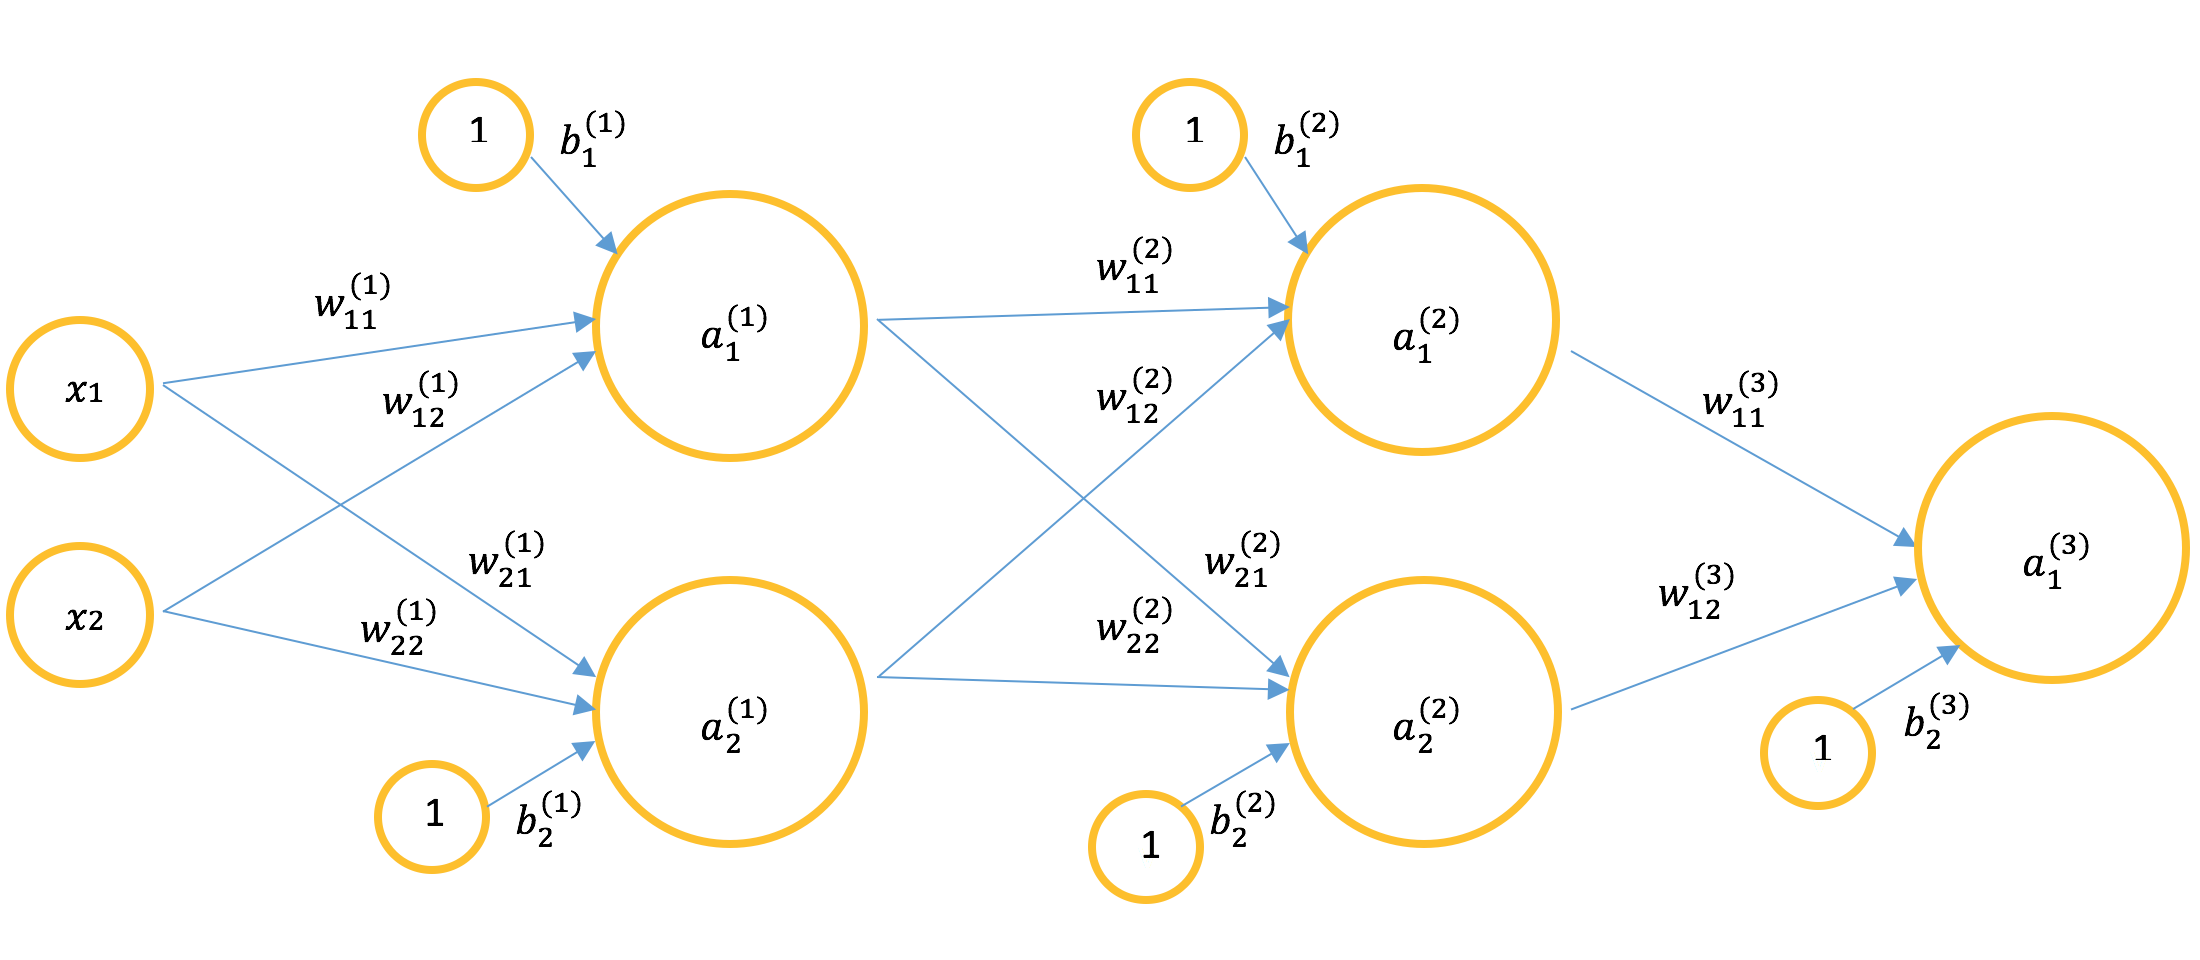
\includegraphics[scale=.3]{neural_net_image.png}
 \end{figure}
 
The notation here is important to keep straight. For the weights the number in the superscript is referring to the current layer, the first number in the subscript is referring to which node the previous node output (or feature) is going to, and the second number in the subscript is referring to which node (or feature) the current weight is coming from. So for example, $w^{(1)}_{12}$ is a weight in the first layer (because of the superscript) and connects the second feature to the first node. 

This notation comes from Nielson's book and helps when we write everything out in matrix multiplication. To see what that looks like for a given layer:

\[
\begin{bmatrix}
           z^{(1)}_{1} \\
           z^{(1)}_{2} \\
           \vdots \\
           z^{(1)}_{m}
         \end{bmatrix}
         =
\left[
  \begin{array}{cccc}
    w^{(1)}_{11} & w^{(1)}_{12} & \hdots & w^{(1)}_{1n} \\
    w^{(1)}_{21} & w^{(1)}_{22} & \hdots & w^{(1)}_{2n} \\
    \hdots &  \hdots  & \hdots &  \hdots \\
    w^{(1)}_{m1} & w^{(1)}_{m2} & \hdots & w^{(1)}_{mn} \\ 
  \end{array}
\right]
\begin{bmatrix}
           x_{1} \\
           x_{2} \\
           \vdots \\
           x_{n}
         \end{bmatrix}
+
\begin{bmatrix}
           b^{(1)}_{1} \\
           b^{(1)}_{2} \\
           \vdots \\
           b^{(1)}_{m}
         \end{bmatrix}
\]

\noindent where $n$ is the number of features, $m$ is the number of nodes, and the $z$'s are the weighted combinations. In shorthand we can write:

\begin{equation}
\mathbf{z}^{(1)} = \mathbf{W}^{(1)} \mathbf{x} + \mathbf{b}^{(1)}.
\end{equation}

One other note to make here is that the bias ($b^{(1)}$) essentially just provides a constant in our linear combination since we are only multiplying it by 1. 

Once this linear combination is fed into the node we pass it through what is known as an activation function. The purpose of this is to help our neural net model nonlinear behavior (see Deep Learning book for further discussion, pages 168-171). Another reason that Nielson points out is that we want a function that provides gradual changes with input. The original perceptron originally outputted a 0 or 1 based on if the weighted combination was greater than some threshold. This is a problem because a slight nudge in one direction could completely flip the neuron and training the network would be harder to do because of neurons that suddenly flip. Some activation functions like the sigmoid essentially approximate the perceptron paradigm (by approximating the step function) but I think the main point is that we want a function that has smoothness properties. The reason we want this is because we can approximate a change in output by a linear combination of the derivatives of the weights and bias with the actual weights and biases implying that the output is a linear function of the inputs and therefore changing parameters becomes more predictable for the algorithm to figure out.

We represent the activation function with $\sigma$ and write the output of the activation function as:
%TODO talk about activation functions here

\begin{equation}
\mathbf{a}^{(1)} = \mathbf{\sigma}(\mathbf{W}^{(1)} \mathbf{x} + \mathbf{b}^{(1)}) = \sigma(\mathbf{z}^{(1)})
\end{equation}
\noindent As Nielson points out we are treating the function $\sigma$ here as a vectorized function. A more explicit way to write this out would be:

\[
\begin{bmatrix}
           a^{(1)}_{1} \\
           a^{(1)}_{2} \\
           \vdots \\
           a^{(1)}_{m}
         \end{bmatrix}
         =
\left[
  \begin{array}{cccc}
    \sigma(w^{(1)}_{11}x_1 & w^{(1)}_{12}x_2 & \hdots & w^{(1)}_{1n}x_n + b_1^{(1)}) \\
    \sigma(w^{(1)}_{21}x_1 & w^{(1)}_{22}x_2 & \hdots & w^{(1)}_{2n}x_n + b_2^{(1)} ) \\
    \hdots &  \hdots  & \hdots &  \hdots \\
    \sigma(w^{(1)}_{m1}x_1 & w^{(1)}_{m2}x_2 & \hdots & w^{(1)}_{mn}x_n + b_m^{(1)} ) \\ 
  \end{array}
\right]
\]

To continue this notation with each subsequent layer we really only need to change a few things. First of all, instead of the original features $x_1, x_2, ..., x_n$ we have $a^{(1)}, a^{(2)}, ..., a^{(m)}$ as the inputs into the next layer. This leads us to change our weight matrix as well so that we have a matrix that is $p$x$m$ where $p$ is the number of nodes in the second layer and $m$ is the number of outputs from layer 1 (before we had $n$ representing the number of \emph{features}). The other thing we need to change is the superscript for the variables such as $\mathbf{W}^{(1)}$ to $\mathbf{W}^{(2)}$ since we are in the second layer. For a generic layer from Nielson's book we can write:

\begin{equation}
\mathbf{z}^{(l)} = \mathbf{W}^{(l)} \mathbf{a}^{(l-1)} + \mathbf{b}^{(l)}.
\end{equation}
\noindent This leads us to also write:

\begin{equation}
\mathbf{a}^{(l)} = \mathbf{\sigma}(\mathbf{z}^{(l)}).
\end{equation}

When designing our networks one heuristic that Nielsen points out is to set the number of nodes to a quantity that actually makes sense. For example, in the recognizing handwritten letters case it is better to have 10 output nodes for digits $0,...,9$ than 4 output nodes outputting a 1 or a 0 (which would allow us to treat the nodes as bits in representing numbers). The first approach might be better because it is directly tied to the images - the output node representing 0 for example should hopefully find information from the other nodes directly from the image to make decisions.


\subsection{Backprop}

Now that we have our notation straight we can talk about how the network is trained using backpropagation. Really at the heart of the backprop algorithm is gradient descent or some iterative optimization technique. To use gradient descent or similar techniques we need to calculate the partial derivatives of what is known as the cost or loss function with respect to the parameters in the model or in the case of neural networks, the weights and biases. Because the neural network is made up of different layers or functions then what this amounts to is using the chain rule for each parameter.

Nielsen brings up two good points with regards to the loss function. Take the common loss function called the mean squared error loss function:

\begin{equation}
C = \frac{1}{2n} \sum_i (y_i - a^{L}(x_i))^2
\end{equation}

First of all, the overall loss function needs to be able to be written as an average of the loss function of separate training examples. This is because backprop is designed to operate one training example at a time (giving us gradients for each training example) and the overall gradient can be recovered by averaging over all the gradients from the training examples as long as our loss function is an average to begin with over all training examples. In practice, averaging the gradient over all training examples is not usually done but instead updates happen in smaller batches called ``mini batches" over a random subset of the data (called stochastic gradient descent). Online learning is when we update after every example.

The second assumption is that the loss function can be written as a function of the outputs of the network. This is just making the point that we want to be able to train the parameters of the model and so the loss function needs to be a function of those parameters.
 
One other note to make is that when doing something like classification, instead of minimizing the classification error directly we minimize the quadratic error in order to make the loss function more smooth which helps us to see better how to change the weights and biases in the right direction.
 
In my mind, it makes sense to think of backprop as a means to an end, in particular finding the gradient at a particular training example. To see this I calculate a partial derivative by hand below and later look at the backprop equations.

 Using our example and notation, lets find the derivative of the function with respect to the weight $w^{(1)}_{12}$. In other words we want to find:
 
 \begin{equation}
\frac{dC_{x_i}}{dw^{(1)}_{12}}.
 \end{equation}
 
\noindent where $C_{x_i}$ is referring to the loss function for a specific training example.
 
\noindent The squared-error loss function for our 3 layered network gives us:
 
 \begin{equation}
 C_{x_i} = \frac{1}{2} {(y_i - a_1^{(3)})^2}
 \end{equation}
 
 \noindent where $a_1^{(3)}$ is the output from the last layer in our example. Note that we are doing this for one particular training example. 
 
 To get at the derivative for $w^{(1)}_{12}$ we rewrite the cost function above with all its nested functions:
 
 \begin{equation}
 \begin{split}
 \frac{1}{2} (y_i - a_1^{(3)})^2 & = \frac{1}{2} (y_i - \sigma(w^{(3)}_{12}a_2^{(2)} + w^{(3)}_{11}a_1^{(2)}+ b_2^{(3)}))^2 \\
 &= \frac{1}{2} (y_i - \sigma(w^{(3)}_{12} \sigma(w^{(2)}_{22}a_2^{(1)} + w^{(2)}_{21}a_1^{(1)}+ b_2^{(2)}) + w^{(3)}_{11}        \sigma(w^{(2)}_{12}a_2^{(1)} + w^{(2)}_{11}a_1^{(1)}+ b_1^{(2)}) + b_2^{(3)}))^2 \\
 &= \frac{1}{2} (y_i - \sigma(w^{(3)}_{12}     \sigma(w^{(2)}_{22}   \sigma(w_{22}^{(1)}x_2 + w_{21}^{(1)}x_1 + b_2^{(1)})    + w^{(2)}_{21}        \sigma(w_{12}^{(1)}x_2 + w_{11}^{(1)}x_1 + b_1^{(1)})+ b_2^{(2)}) \\
 &+ w^{(3)}_{11}        \sigma(w^{(2)}_{12}  \sigma(w_{22}^{(1)}x_2 + w_{21}^{(1)}x_1 + b_2^{(1)})  + w^{(2)}_{11} \sigma(w_{12}^{(1)}x_2 + w_{11}^{(1)}x_1 + b_1^{(1)})+ b_1^{(2)})     + b_2^{(3)}))^2
 \end{split}
 \end{equation}

We then use the chain rule to get:

\begin{equation}
\frac{dC}{dw^{(1)}_{12}} = (y_i - a_1^{(3)})(-\sigma^\prime(z_1^{(3)}))[w_{12}^{(3)}\sigma^\prime(z_2^{(2)})w_{21}^{(2)}\sigma^{\prime}(z_1^{(1)})x_2 + w_{11}^{(3)}\sigma^{\prime}(z_1^{(2)})w_{11}^{(2)}\sigma^{\prime}(z_1^{(1)})x_2].
\end{equation}

We can do this for all partial derivatives with respect to our parameters (the weights and biases) giving us our gradient $\nabla C_{x_i}$ which is used in the gradient descent equation:

\begin{equation}
\theta_t = \theta_{t-1} + \eta \left( -\nabla C_{x_i}(\theta_{t-1}) \right).
\end{equation}
In this equation $\theta_t$ represents the parameters to the neural network at iteration $t$, $C_{x_i}$ represents our cost function for training example $i$, and $\eta$ is the learning rate. This update equation implies that we are updating after each training example which might not be ideal.

It is key to remember that we are treating the loss function as a function of $\theta$ and keeping everything else fixed. The goal is to find the $\theta$ that minimizes the overall loss function.


As we can see from the previous section, the algebra for this can get lengthy and messy. A key turning points for neural networks was finding a quicker way of calculating partial derivatives. 

In terms of the same weight we found above ($w^{1}_{12}$) we have the four backprop equations. Equation 1 is the error of the $j^{th}$ node in the last layer:

\begin{equation}
\delta^{L}_j = \frac{dC}{da^L_j} \sigma^\prime(z_j^L)
\end{equation}

\noindent Breaking this down we see that the first quantity on the right side of the equation is letting us know how fast the cost function is changing with respect to the output of the $j^{th}$ node. If this is high, then we know that the cost function is still fluctuating rapidly along this direction and we aren't at a minimum yet with respect to that direction. In this sense we can think of $\delta{L}_j$ referring to the error of the node. We can also write this all in vectorized form $\delta^{L}$.

Nielsen shows that the fourth backprop equation is:


\begin{equation}
\frac{dC}{dw^{(1)}_{12}} = a_{2}^{0}\delta_1^{(1)}
\end{equation}
which we can then use the other equations to recursively get at the other $\delta$'s.

The quantity $\delta_1^{(1)}$ is given by:

\begin{equation}
(w_{11}^{(2)}\delta^{(2)}_1 + w_{21}^{(2)}\delta^{(2)}_2)\sigma^{\prime}(z_1^{(1)})
\end{equation}
 
 We then recursively get the other $\delta$'s in the equation:
 
 \begin{equation}
 \begin{split}
 \delta^{(2)}_1  & = w_{11}^{(3)}\delta_1^{(3)}\sigma^{\prime}(z_1^{(2)})\\
 \delta^{(2)}_2  & = w_{12}^{(3)}\delta_1^{(3)}\sigma^{\prime}(z_2^{(2)})
 \end{split}
 \end{equation}

What makes the backprop algorithm so fast is that we can compute all of the partial derivatives with one forward and backward pass, whereas other methods require multiple passes. 
 
One other note to make is that nodes can become saturated when using activation functions like the sigmoid because the derivative will be close to zero on the edges of that function. When that happens then the update in the gradient descent formula will be minimal.

Hyperparameter tuning is where the magic or art of neural nets occur. There are heuristics we can learn.

 
 
 
 \subsection{Recurrent and Recursive Nets}
 
(Notes from Deep Learning Book)

\begin{itemize}
\item Recurrent Nets (RNNs) are built to handle a sequence of values $\mathbf{x}^{(1)},..., \mathbf{x}^{(\tau)}$
\item Main idea is of sharing parameters across different parts of the model which allows us to deal with different sequence lengths. This is contrasted with a regular neural network which would have a separate parameter for each word position in a sentence. If the sentence has the same meaning, but is out of order we could get a totally different answer.
\item A related idea for sharing parameters is by using a neighborhood around the \emph{inputs}. With RNNs however each member of the output is a function of previous members of the \emph{output}.
\item We define hidden units as $\mathbf{h}^{(t)} = f(\mathbf{h}^{(t-1)}, \mathbf{x}^{(t)}; \theta)$. If we are trying to predict the future from the past (predict the next word given a sequence of words) then $\mathbf{h}^{(t)}$ provides a type of lossy summary of the previous inputs up to $t$. 

\item Teacher forcing is where you take the target value of one time step and input it into the next time step

\end{itemize}
 

\section{Unsupervised}
\subsection{Principal Components Analysis}

Principal Components Analysis (PCA) is one of the most common ways of reducing dimension of a dataset. The main algorithm is as follows:

\begin{enumerate}
\item Standardize dataset that we want to perform PCA on. This entails subtracting the mean and dividing by the standard deviation.

\item Get covariance matrix of dataset.

\item Do eigen value decomposition on covariance matrix.

\end{enumerate}


If we have our data matrix $X$ which is $n$x$p$ ($n$ number of instances, $p$ number of features), then our correlation matrix is given by:

\begin{equation}
\frac{1}{n}X_s^TX_s
\end{equation}

\noindent where $X_s$ is the standardized matrix (subtract the mean and divide by standard deviation for each feature). 



\section{Basic Probability}
\input{probability}

\section{Classical Statistics}
\subsection{Statistical Tests}

Perhaps the most important concept or theoretical underpinning of all of classical statistics is the Central Limit Theorem. This theorem states that for a random sample $X_1, X_2, ..., X_n$, which is identically and independently distributed with mean $\mu$ and standard deviation $\sigma$, the sample mean is approximately distributed as such:

\begin{equation}
\bar{X} \sim N(\mu, \frac{\sigma^2}{n})
\end{equation}

\noindent where $\bar{X}$ is the sample average and as n goes to infinity.

Many of the classical significance tests in statistics are based off of this theorem. For example, say we want to understand if the true mean of a population is different than zero for some scenario. We would set up the test by first defining the null and alternative hypotheses:

\begin{equation}
\begin{split}
H_0 &: \mu = 0 \\
H_A &:  \mu \neq 0
\end{split}
\end{equation}

\noindent Since we can't know the true population mean (we can't survey the entire population for example) we are limited to a random sample and the mean of that sample. However, we don't want to make a conclusion based solely off the sample mean because of the variability that is introduced by the random sample. For example, say the sample mean is 1. One conclusion (possibly false) we could make is that the population mean must be close to 1 as well and therefore we would reject the null hypothesis. Its possible however, due to chance we got a sample that happened to have a mean of 1 whereas the population mean is really 0.

To account for this issue we use the central limit theorem to imagine a \emph{sampling distribution} where we take many, many samples of size $n$ from the original population and plot the means to form a distribution. This distribution according to the CLT will be distributed $N(\mu, \frac{\sigma^2}{n})$. Using our given sample, we temporarily make the assumption that the null hypothesis is true ($\mu=0$) and figure out how many standard deviations away our sample mean $\bar{X}$ is from $\mu=0$. This is the z-score.

Before doing this test we decide on a threshold we are comfortable with for determining if the z-score is too ``far'' away from the mean to be due to just chance. One way to express this threshold is through an alpha value, such as $\alpha=0.05$. If we find that the probability under the sampling distribution of the sample mean being as extreme or more extreme than the derived z-statistic is greater than $\alpha=0.05$, we fail to reject the null hypothesis and say ``this sample mean is close enough to 0 so we will call the population mean 0". If the same probability is less than 0.05 we reject the null hypothesis, accept the alternative, and say ``this sample mean was so far away from 0 it must not be due to chance". 

The probabilities above are known as p-values. It is key to remember that the interpretation of a p-value is not the probability of the null hypothesis being true. It is the ``probability, under the null hypothesis, that we get a value as extreme or more extreme than the one observed".

Below are common statistical tests that make use of this entire framework, but with different variations. I attempt to summarize the most important tests and guiding rules to know which ones should be used under different circumstances.
\newline

\noindent \underline{\textbf{One sample z-test}}:

The equation for the one sample z-test is given by:
\begin{equation}
z = \frac{\bar{X} - \mu}{\frac{\sigma}{\sqrt{n}}}
\end{equation}

Often times $\sigma$, the population standard deviation, is not known so we instead replace it with $s$, the sample standard deviation. As a rough rule, if $n>30$, we say the sample standard deviation approximates the population standard deviation close enough and we feel more confident in treating the sampling distribution as normal. This is a rough rule so it seems when in doubt it is better to use the t-score. 

The conditions for using the z-score are therefore:
\begin{itemize}
\item Random sample
\item Independence condition (the individual observations in the sample are independent)
\item Normal condition (underlying population is normal or the sample size is large enough meaning $n>30$). If $n<30$ we need to look at the underlying data to see if the distribution is skewed or if there are outliers. If not then it may be safe to assume the sampling distribution will be normal. Note here as well that for proportions (when our original data is binary and we are doing a hypothesis test on the proportions) the test for normality is $np, n(1-p) > 10$.
\end{itemize}

\noindent \underline{\textbf{One sample t-test}}:
The equation for the one sample t-test is given by:
\begin{equation}
t= \frac{\bar{X} - \mu}{\frac{\sigma}{\sqrt{n}}}
\end{equation}

This is the same as the z-test but we use this test if we see that the population distribution is not normal and $n<30$ (as a general rule of thumb). Again if we don't know the population standard deviation we replace $\sigma$ with $s$. The other conditions (random sample and independence conditions described above) should be met as well.
\newline

\noindent \underline{\textbf{Two sample z-test}}:
Two sample tests are used to compare the means of two random and independent samples. The results are similar but instead of imagining a sampling distribution of $\bar{X}$, we instead imagine a sampling distribution of $\bar{X}_1 - \bar{X}_2$. This sampling distribution is found by first imagining the separate sampling distributions for $\bar{X}_1$ (mean $\mu_1$ and standard deviation $\frac{\sigma_1}{\sqrt{n_1}}$) and $\bar{X}_2$ (mean $\mu_2$ and standard deviation $\frac{\sigma_2}{\sqrt{n_2}}$). The mean therefore of $\bar{X}_1 - \bar{X}_2$ will be $\mu_1 - \mu_2$ and the standard deviation will be

\begin{equation}
\begin{split}
\sqrt{\text{Var}(\bar{X}_1 - \bar{X}_2)} & = \sqrt{\text{Var}(\bar{X}_1 + (- \bar{X}_2))} \\
&=\sqrt{\text{Var}(\bar{X}_1) + (-1)^2 \text{Var}(\bar{X}_2) + (-1)*2\text{Cov}(\bar{X}_1, \bar{X}_2)} \\
&=\sqrt{\text{Var}(\bar{X}_1) + \text{Var}(\bar{X}_2)}  \hspace{1em}   \text{(since $\bar{X}_1$ and $\bar{X}_2$ are independent)}\\
&=\sqrt{ \frac{\sigma_1^2}{n_1} + \frac{\sigma_2^2}{n_2}}
\end{split}
\end{equation}

Our null hypothesis will then typically be:

\begin{equation}
\begin{split}
H_0 &: \mu_1 - \mu_2 = 0 \\
H_A &:   \mu_1 - \mu_2 \neq 0
\end{split}
\end{equation}

\noindent If both samples are large enough ($n_1, n_2 > 30$) then we assume that the sampling distribution of $\bar{X}_1$ - $\bar{X}_2$ is normal and we can use the z-score:

\begin{equation}
z = \frac{(\bar{X}_1 -   \bar{X}_2) - (\mu_1 - \mu_2)}{\sqrt{\frac{s_1^2}{n_1} + \frac{s_2^2}{n_2}}}.
\end{equation}

\noindent \underline{\textbf{Two sample t-test (variances are different)}}:

If the one of the sample sizes is below 30 then it is best to use the t-test. The score below is used when the variances are different. This is known as Welch's t-test:

\begin{equation}
t = \frac{(\bar{X}_1 -   \bar{X}_2) - (\mu_1 - \mu_2)}{\sqrt{\frac{s_1^2}{n_1} + \frac{s_2^2}{n_2}}}.
\end{equation}

\noindent \underline{\textbf{Two sample t-test (variances are same)}}:

\begin{equation}
t = \frac{(\bar{X}_1 -   \bar{X}_2) - (\mu_1 - \mu_2)}{s_p\sqrt{\frac{1}{n_1} + \frac{1}{n_2}}}.
\end{equation}


\subsection{Analysis of Variance (ANOVA)}

The previous test statistics are for when we want to compare a sample mean with some value or when we want to compare two sample means with each other. Analysis of Variance comes into play when we want to compare multiple samples (3 or more). 















\section{Natural Language Processing}
\subsection{Tf-idf}

Term frequency - inverse document frequency (tf-idf) is a metric that attempts to measure how important a word is to a document. It increases proportionally for a particular word as the number of times the word appears in a document increases, but decreases if that word appears in multiple documents within a corpus. This helps to account for words that appear regularly in language. 

A basic implementation of tf-idf is given by the following. First find the term frequency function:

\begin{equation}
\text{tf}(t,d) = f_{t,d}
\end{equation}
\noindent where $t$ is the term we are assessing, $d$ is a particular document, and $f_{t,d}$ is the simple count of the number of times $t$ appears in the document $d$. We can use other schemes in place of $f_{t,d}$; this is one of the more simple implementations.

The inverse document frequency part can be written as the following:

\begin{equation}
\text{idf}(t,D) = \log{\frac{N}{|\{d \in D:t\in d \}| }}
\end{equation}
\noindent where $D$ is the corpus, $N$ is the number of documents in the corpus, and $|\{d \in D:t\in d \}|$ is the number of documents the term $t$ appears in. Again, there are other metrics than can be used in place of this function but the idea remains roughly the same. 

To get the complete metric we multiply the tf part together with the idf part. 


\subsection{Skip-gram}

The main idea in the Skip-gram approach is to use a simple neural network to find vector representations of words that encode context or a better way to say it is representations ``that are useful for predicting the surrounding words in a sentence or document" (source Distributed Representations of Words and Phrases and their Compositionality). 

The way this is done is to take all the words in a sentence or document and encode them as one-hot vectors. The length of these vectors will be equal to the number of words in the document. Training examples are then built by creating tuples of words that appear next to each other. So given the phrase ``the quick brown fox", we generate training examples (``brown", ``quick") and (``brown", ``fox") or in their encoded vector form $([0,0,1,0],[0,1,0,0])$ and $([0,0,1,0],[0,0,0,1])$. 

We then pass these training examples into a single layer neural network with no activation functions. Because we are passing in a one-hot vector this essentially slices a column of the weight matrix, and inputs into the single hidden layer. If, for example, we have 300 hundred hidden nodes and 10,000 words in our document, then our weight matrix will be $300x10,000$ and a slice of the weight matrix will be a vector of size 300. I'm assuming we still include bias in the hidden layer? 

The second layers weight matrix will then be $10,000x300$, outputting a 10,000 length vector. The softmax function is used on the resulting vector which is defined as:

\begin{equation}
\sigma(\mathbf{z})_i = \frac{e^{z_i}}{\sum_{j=1}^{K}e^{z_j}} 
\end{equation}
\noindent for $i=1,...,K$ and $\mathbf{z} = (z_1, ...,z_K)$.

In words, this function takes in a vector and outputs a vector of the same size, but where each element is exponentiated and divided by the sum of all other elements exponentiated. This new vector is therefore a discrete probability distribution. The name \emph{softmax} comes from the concept that the function is attempting to approximate the arg max function. A better name would probably be the softargmax function, but softmax is commonly used.

Comparing the softmax output with the training label (the one-hot encoded word in the bigram associated with our input) and using gradient descent, will change the weights of the neural network in such a way that the softmax output will converge towards a vector with higher probability on the element associated with 1 in the training label's one-hot vector. The balance to this however, it that a particular training input will have multiple training labels because of the different bigrams, and so the probabilities will change for different elements, forcing the weights to account for the context of words and to encode each word. Another thought about this is that if we were to input the same word as we are trying to predict, then our output layer weight matrix will adjust the weights in the corresponding row in such a way that forces the softmax output to be as close to 1 as possible. However, because we are putting in different words, the corresponding row in the weight matrix will balance the different words to encode context.

In summary, the second layer's weight matrix will provide the 300 length vector representation of each of the 10,000 words. If we wanted to vector representation of the first word in the vocabulary, we would take the first row of the weight matrix. Its important to remember that the output of this whole process is not the model itself but the weight matrix giving us the vector representations. This means we can essentially have a pre-trained dictionary of vector representations, but only for words that were in our original model training. Implementations like FastText however, do something that encodes subwords and so we can actually get vector representations for words the model has never seen. 

The paper ``Distributed Representations of Words and Phrases and their Compositionality" does a couple of things that make the training easier such as removing common words like ``the", putting common phrases together as one word, and doing a process called negative sampling where we only have say 6 output nodes where 5 of them are negative examples and one of them is the true example. This greatly reduces the scale of the problem.

\subsection{Continuous Bag of Words (COBW)}

This is almost the same approach as the Skip-gram model, but instead of passing in tuples to the model we pass in a sentence, or group of words (order doesn't matter hence the term ``bag of words"), that surround the word of interest, and allow this word of interest to be the target value in the model. Each word in the group of words is one-hot encoded and then all one-hot encoded vectors are averaged together. At this point we proceed as before with the Skip-gram model, but with an input vector that is less sparse. This approach creates vectors that represent the target words, but that also encodes the context of the sentence or group of words that are passed in. 

COBW is faster, but Skip-gram does better on less frequent words (see \href{https://code.google.com/archive/p/word2vec/}{here}). Also see this \href{http://mccormickml.com/2016/04/19/word2vec-tutorial-the-skip-gram-model/}{tutorial} I used for a more intuitive understanding of word2vec.

\subsection{Latent Dirichlet Allocation}

The majority of this section comes from the original paper ``Latent Dirichlet Allocation" by Andrew Ng, Michael Jordan, and David Blei and a lab from the applied math program at BYU found \href{http://acme.byu.edu/wp-content/uploads/2019/01/GibbsSampling.pdf}{here}.

Assume we have a vocabulary set of size $V$ (meaning we consider $V$ number of words), a corpus size of $M$, (meaning we have $M$ different documents), and $K$ different topics. 

LDA is a generative model process where we assume a process that ``generates" our documents and words. The BYU ACME lab does a good job of outlining this process:

\begin{enumerate}
\item Choose $\phi_k \sim  \text{Dir}(\beta)$ for $1 \leq k \leq K$
\end{enumerate}
For $1 \leq m \leq M$:
\begin{enumerate}
\item Choose $\theta_m \sim \text{Dir}(\alpha)$
\item Choose $z_{m,n} \sim  \text{Cat}(\theta_m)$ for $1 \leq n \leq N_m$
\item Choose $w_{m,n} \sim  \text{Cat}(\phi_{z_{m,n}})$ for $1 \leq n \leq N_m$
\end{enumerate}
\noindent In words the first step is to draw probability vectors $\phi_k$ of length $V$ for each topic $k$. Draws from a Dirichlet distribution return a vector of probabilities, essentially the multi-variate version of the beta distribution. This vector encodes the way each topic is represented by the vocabulary of $V$ words.

The next step is to generate the $M$ documents. This is done by again drawing from the Dirichlet distribution, but this time taking a vector of length $K$ ($\theta_m$) and thereby encoding the way the $m^{th}$ document is represented by the $K$ topics. In other words, this vector gives us the probabilities that the $m^{th}$ document is assigned to topic $k$. 

We then pass the $\theta_m$ vector into a categorical distribution and repeat $N_m$ times, giving us $N_m$ integers that represent each topic, where the probabilities of the categorical distribution are given by $\theta_m$. The last step is to draw $N_m$ words $w_{m,n}$ from another categorical distribution, which this time is parameterized by $\phi_{z_{m,n}}$, or the probability vector for the $z_{m,n}^{th}$ topic.


\section{Problems}
Below are probability questions that I've collected. Their answers appear in the following subsection.

\subsection{List of Problems}

\begin{enumerate}
\item[1.1] What is the random variable and associated pdf and cdf of the following experiment - ``toss a coin until a head appears". Also prove that the cdf is a true cdf.

\item[1.2] Say we have a standard normal distribution that we take draws from $X_1, X_2, ...$ until we draw a value that is greater than some value $p$, in which case we stop sampling. What is the expected value of the draws?

\item[1.3] Find the probability that two points on a unit line have a distance less than 0.5. What is the probability that two random points on the border of a unit square is less than 0.5?

\item[1.4] Given the joint distribution $f(x,y) = e^{-y}$ with support $0<x<y< \infty$ find the marginal distribution of $X$, the marginal distribution of $Y$ and $P(X+Y<1)$.

\item[1.5] What is the distribution of the sum of two independent Poisson random variables, $X$ and $Y$?

\item[1.6] If $X \sim N(\mu_1, \sigma_1)$ and $Y \sim N(\mu_2, \sigma_2)$ are independent what is $Z=X+Y$ distributed as?

\item[1.7] The birthday problem - what is the probability in a room full of $n$ people that there is at least one pair that share the same birthday?

\item[1.8] A probability of success in a trial is given by $p$. For two trials, what is the probability I get two successes, given that at least one of them is a success. 

\item[1.9]
You will flip 8 fair coins in total and you've already flipped 4 of them. 3 of them have come up with tails. What is the expected number of tails by the time you've flipped all of them?

\item[1.10]
Kenzie has a 6 sided die with values 3,3,3,3,6,6 and Matt has a die with values 2,2,2,5,5,5. If they each roll the die at the same time and winner is the one with the highest number, who will win the most games in the long term?

\item[1.11]
If I get heads I put a red ball in a bag. If I get tails I put a blue ball in a bag. I do this two times so I have two balls in a bag. I then pick a ball out randomly and get a red ball. I put it back. What is the probability I chose a blue ball the second time?

\item[1.12]
Say we have 10 doors with a car behind one door. You choose one door and the game show host opens 8 other random doors. What is the probability that the car is behind the door he didn't open?

\item[1.13]
What is the probability of choosing four of a kind from a 52 card deck? (4 spades, 4 hearts, etc.). What is the probability of choosing one of each kind?

\item[1.14]
Bobo the amoeba can have zero children (with .25 prob), one child (.25), or two children (.5). What is the probability that his lineage dies out?

\item[1.15]
Imagine I have two scenarios - one where the probability of pushing a button once gives me an electrical shock with probability 0.9 and the other one where the button gives me a shock with probability 0.1 but I push it 10 times. Which scenario is better for me?

\item[1.16]
What is the probability of getting at least an 80 percent on a true false test with 20 questions if we just randomly guess?

\item[1.17]
My telephone rings 12 times each week, the calls are randomly distributed across the 7 days. What is the probability I get 4 calls one day, 2 calls on each of two days and 1 call on each remaining day?

\item[1.18]
A textbook has $n$ typos randomly scattered across $n$ pages. If we pick a random page what is the probability there are no typos on it?

\item[1.19]
In a group of $n$ people, what is the expected number of distinct birthdays (month and day)? What is the expected number of birthday matches?

\item[1.20]
There are n people at a party, each with hat. At the end of the party, they each leave with a random hat. What is the expected number of people who leave with the right hat?

\item[1.21]
In any 15-minute interval, there is a 20\% probability that you will see at least one shooting star. What is the probability that you see at least one shooting star in the period of an hour?

\item[1.22]
How can you generate a random number between 1 and 7 using a normal die?

\item[1.23]
If someone gives you a unfair coin how do you get a fair outcome from it?

\item[1.24]
You have a group of couple that decide to have children until they have their first girl, after which they stop having children. What is the expected number of children each couple will have?

\item[1.25]
How many ways can you split 12 people into 3 teams of 4?

\item[1.26]

We have a hash function that maps 10 object to elements 1-10 (inclusive), with equal probability. What is the probability of a hash collision? What is the expected number of hash collisions? What is the expected number of hashes that are unused?

\item[1.27]
You call 2 Ubers and 3 Lyfts where the time it takes for them to show up is iid. What is the probability that the first 3 that show up are Lyfts? What about for Uber?

\item[1.28]

A lazy high school senior types up n applications to colleges but randomly puts them in n envelopes addressed to each college. Whats the expected number of colleges that will get the correct applications?

\item[1.29]

What’s the expected number of coin flips until you get two heads in a row? What’s the expected number of coin flips until you get two tails in a row?

\item[1.30]

Let’s say we play a game where I keep flipping a coin until I get heads. If the first time I get heads is on the nth coin, then I pay you 2n-1 dollars. How much would you pay me to play this game?

\item[1.31]
You have a 0.1\% chance of picking up a coin with both heads, and a 99.9\% chance that you pick up a fair coin. You flip your coin and it comes up heads 10 times. What’s the chance that you picked up the fair coin, given the information that you observed?

\item[1.32]

A certain couple tells you that they have two children, at least one of which is a girl. What is the probability that they have two girls? What if I say that the oldest child is a girl what is the probability both are girls then?

\item[1.33]
I write a program should print out all the numbers from 1 to 300, but prints out Fizz instead if the number is divisible by 3, Buzz instead if the number is divisible by 5, and FizzBuzz if the number is divisible by 3 and 5. What is the total number of numbers that is either Fizzed, Buzzed, or FizzBuzzed?

\item[1.34]
This problem is commonly known as the coupon collector problem. There are n coupon types. At each draw, you get a uniformly random coupon type. What is the expected number of coupons needed until you have a complete set?


\end{enumerate}

\subsection{Answers}

\begin{enumerate}

\item[1.1] What is the random variable and associated pdf and cdf of the following experiment - ``toss a coin until a head appears". Also prove that the cdf is a true cdf.

First of all we recognize that this is a geometric distribution which counts the number of failures until the first success. The geometric pmf is given by:

\begin{equation}
q^{x}p
\end{equation}

\noindent where $q$ is the probability of failure, $p$ is the probability of success, and $x$ is the number of failures. The support is on all nonnegative integers. 

We note that the pmf gives the distribution of number of failures whereas we want to include the time the coin actually appears heads. Therefore we want $x+1$. This requires a transformation where $g(X) = X + 1$.

Using equation \ref{eq:pmf_transform} we have for $Y=g(X)$ and $g^{-1}(Y) = Y - 1$:

\begin{equation}
f_Y(y) = \sum_{x \in g^{-1}(y)} P(X = x) = \sum_{x \in g^{-1}(y)} q^{x}p = q^{y-1} p
\end{equation}
\noindent The last step occurs because $g$ is a one-to-one function and the only $x$ that maps to our $y$ is $y-1$. 

Now that we have our pmf, we want to find the cdf. This is done by doing the following

\begin{equation}
F_Y(y) = P(Y \leq y ) = \sum_{i=1}^{y} (1-p)^{i-1}p  = p \left [ \frac{1 - (1-p)^y}{1 - (1-p)} \right ] = 1 - (1-p)^y
\end{equation}
\noindent by the geometric series.

To prove this is a cdf we show that as $y$ goes to $-\infty$ we get 0 (which is true because $F_Y(y)$ is defined to be 0 for $y<0$, as it goes to $\infty$ we get 1 (which is true because $1-p$ is a number less than 1 and raised to infinity goes to 0), it is monotonically increasing, and lastly we show it is right continuous by $F_Y(y+\epsilon) = F_Y(y)$ as $\epsilon$ goes to 0. 



\item[1.2] Say we have a standard normal distribution that we take draws from $X_1, X_2, ...$ until we draw a value that is greater than some value $p$, in which case we stop sampling. What is the expected value of the draws?

The first step is to write down what we want. The way to think of this is that we want to know the expected value of $X$ (where $X$ is a normal random variable), but with the condition that $X<p$. This can be written as $ E[X|X<p]$. Using the standard normal distribution we have:


\begin{align*}
E[X|X<p] &= \int_{-\infty}^{\infty} x f_X(x|X<p) dx \hspace{2em}  \text{(by definition of expectation)}\\ 
&=  \int_{-\infty}^{\infty} x \frac{f_X(x, X<p)}{P(X<p)} dx  \hspace{2em} \text{(by definition of conditional probability)} \\
&= \frac{1}{P(X<p)} \int_{-\infty}^{p} x \frac{1}{\sqrt{2\pi}}e^{\frac{-x^2}{2}} dx \hspace{2em} \text{(limit integral bounds to match conditional prob.)} \\
&= \frac{1}{P(X<p)\sqrt{2\pi}} \int_{-\infty}^{p} x e^{\frac{-x^2}{2}} dx
\end{align*}

\noindent The quantity $P(X<p)$ is given by the cdf of the standard normal distribution. The integral, using u-substitution, is found to be:

\begin{equation}
\begin{split}
\int_{-\infty}^{p} x e^{\frac{-x^2}{2}} dx  &= \int_{-\infty}^{\frac{-p^2}{2}} - e^{u} du \\
&= -e^{\frac{-p^2}{2}} + e^{-\infty} \\
&= -e^{\frac{-p^2}{2}}
\end{split}
\end{equation}
\noindent where $u=\frac{-x^2}{2}$.

All together we have $\frac{-e^{\frac{-p^2}{2}}}{P(X<p)\sqrt{2\pi}}$. If $p=1$ for example then we have 

\begin{equation}
\frac{-e^{\frac{-1}{2}}}{P(X<1)\sqrt{2\pi}} \approx \frac{-e^{\frac{-1}{2}}}{0.84*\sqrt{2\pi}} \approx -0.288
\end{equation}


One question I had is if there is a difference between taking the expectation of a sequence from the distribution and stopping once we have a value that is greater than $p$ vs. taking the expectation of a set sample with variables that are greater than $p$ thrown out. 

From a simulation perspective there is no difference if we think of the set sample as a bunch of sequences tied together, broken up by the values greater than $p$. In this light, the sequences are essentially defined by the realizations that are greater than $p$. So even though thinking about this process from a sequence point of view, I feel it is safe to conclude that we are just taking the normal random sample process approach, looking for the expectation of $X$ conditioned on the event that $X<p$. 

The code for this simulation is given below:

\begin{lstlisting}[language=Python]
from scipy.stats import norm
import numpy as np

mean_rvs = []
N = 10000
p = 1
for i in range(N):
    rvs = []
    less = True
    while less:
        rv = norm.rvs(size=1) # sample one normal, standardized random variable
        if rv < p: # if draw is less than p, add to sequence
            rvs.append(rv[0])
        else: # if draw is greater than p, stop sequence
            less=False
    if len(rvs)!=0: # take mean of sequence, as long as there is as least one random variable in sequence
        mean_rvs.append(np.mean(rvs))
\end{lstlisting}
\noindent where the mean of ``mean\_rvs'' is around -0.288.


\item[1.3] Find the probability that two points on a unit line have a distance less than 0.5. What is the probability that two random points on the border of a unit square is less than 0.5?


\begin{equation}
\begin{split}
P(|Y-X| < 0.5) &= P(-0.5 < Y-X < 0.5) \\
&= P(Y-X < 0.5) - P(Y-X < -0.5) \\
&= P(Y < X + 0.5) - P(Y < X - 0.5)
\end{split}
\end{equation}

We can think of $Y, X$ having a joint uniform distribution on the unit square. This gives us every possible combination of these two variables. If we think of it in this context and relate the two variables together then we can deal with the probability terms above. 

The first part of the last expression above is going to be the area (since this is the uniform distribution) below the line $Y = X + 0.5$ on the unit square. This ends up being $\frac{7}{8}$. The second part will be the area below the line $Y < X - 0.5$ which ends up being $\frac{1}{8}$. Therefore we have a difference of $\frac{6}{8}$ or 0.75. 

The second part to this question requires knowing the probability of two points in general on the unit square having a distance less than 0.5. To answer this assume that one point falls on the bottom of the box and the other on the right of the box. We can then use the pythagorean theorem to get:

\begin{equation}
\begin{split}
P(\sqrt{(1-X)^2 + Y^2} < 0.5) &= P((X-1)^2 + Y^2 < 0.25) 
\end{split}
\end{equation}
\noindent We can recognize this quantity within the probability as the equation of a circle where the center is at $(1,0)$. If we draw this on the unit square and find the area of the intersection we see that the probability is $\frac{\pi}{16}$ (we need to just find the area since it is distributed uniformly, if it were another distribution we would need to actually do an integral.) 

We find that no matter which two adjacent sides the points are on we will still have a probability of $\frac{\pi}{16}$. 

At this point we want to use the law of total probability to split up the event $A$ where $A$ equal ``the probability two points on a unit square are less than 0.5'':

\begin{equation}
\begin{split}
P(A) &= 4*P(A|B)P(B) + 8*P(A|C)P(C)
\end{split}
\end{equation}
\noindent I've obviously skipped some steps here but the ideas is this: if we choose random two points on the unit square then there is a $\frac{1}{16}$ chance they appear on the same side which is what $P(B)$ is representing. We already know $P(A|B)$ is 0.75 from the previous discussion and we multiply it by 4 since there are 4 sides. One thing I was confused on is why we don't multiply it by 8 since the points could be reversed but if we think of assigning two points to the four different sides and every possible combination this would be double counting a combination.

The second part of the equation shows the probability of two points being on adjacent sides $P(C)$ which is also $\frac{1}{16}$ and we know that $P(A|C)$ is $\frac{\pi}{16}$. We multiply by 8 since there are 4 possibilities of adjacent sides and where each point could be switched leading to 8 cases. 

I've omitted the last case where the points are on opposite sides since these distances will be larger than 1 so the probability of it being less than 0.5 is 0.

Adding this all up we get around 0.28567.

I verify this in simulation code below:

\begin{lstlisting}[language=Python]
sim_size = 200000
distances = np.zeros(sim_size)
for i in range(sim_size):
    x = np.random.uniform(0,4.0)
    y = np.random.uniform(0,4.0)

    if x <= 1.0:
        point_x = (x,0.)
    elif x > 1.0 and x<=2.0:
        point_x = (1.,x-1)
    elif x > 2.0 and x <= 3.0:
        point_x = (1-(x-2), 1.)
    else:
        point_x = (0, 1-(x-3))
        
    if y <= 1.0:
        point_y = (y,0.)
    elif y > 1.0 and y<=2.0:
        point_y = (1.,y-1)
    elif y > 2.0 and y <= 3.0:
        point_y = (1-(y-2), 1.)
    else:
        point_y = (0, 1-(y-3))
    
    distances[i] = la.norm(np.array(point_x) - np.array(point_y))
    
sum(distances <.5)/(sim_size*1.0)
\end{lstlisting}


\item[1.4]
Given the joint distribution $f(x,y) = e^{-y}$ with support $0<x<y< \infty$ find the marginal distribution of $X$, the marginal distribution of $Y$ and $P(X+Y<1)$.

The best approach to these problems is to visualize the support as in Figure \ref{fig:support}. To find $P(X+Y<1)$ we can rearrange the equation to equal $P(Y<1-X)$. The way to think of this quantity is the probability of an event $Y<1-X$ which is the integral of the pdf over every possible $Y,X$ in the support and that satisfies the above equation. This limits our integral to the support found in Figure \ref{fig:support2}. 

 \begin{figure}[t] \label{fig:support}
\caption{Support for joint probability function $f(x,y) = e^{-y}.$}
\centering
 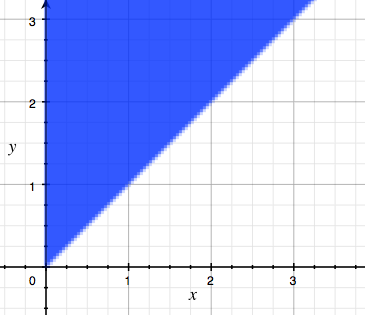
\includegraphics[scale=.7]{support.png}
 \end{figure}
 
  \begin{figure}[t] \label{fig:support2}
\caption{Area to integrate over}
\centering
 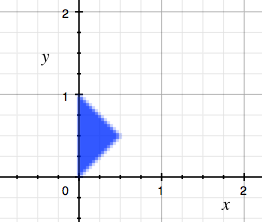
\includegraphics[scale=.7]{support2.png}
 \end{figure}
 
 
 Our integral therefore is:
 
 \begin{equation}
 \begin{split}
 \int_0^{0.5}{\int_x^{1-x}{e^{-y}dy}dx} &= \int_0^{0.5}{-e^{-1+x} + e^{-x}dx} \\
& =  -e^{-1+0.5} - e^{-0.5} + e^{-1} + 1 \\
& \approx 0.1548181217
 \end{split}
 \end{equation}
 
 To find the marginal of $X$ we take the integral over all $Y$:
 
 \begin{equation}
 \int_x^{\infty}{e^{-y}dy}
 \end{equation}
 
 \noindent To find the marginal of $Y$ we take the integral over all $X$:
 
 \begin{equation}
 \int_0^{y}{e^{-y}dx}.
 \end{equation}
 
 
\item[1.5] \label{item:sum_possion}

What is the distribution of the sum of two independent Poisson random variables, $X$ and $Y$?

If we take the bivariate transformation approach we want one variable to be the sum of $X$ and $Y$ so that we can marginalize the other variable out to get this distribution. Therefore we let $U=X+Y$ and $V=Y$. The support of $X$ and $Y$ are the non-negative integers so the support of $V$ will be the same and the support of $U$ will be $v, v+1, ...$ since $u=x+v$.

When determining which values $(x,y)$ we need to sum over for each $(u,v)$ we ask for any $(u,v)$ pair what are the $(x,y)$ values that give me that pair or in other words what $(x,y)$ values solve both equations? The answer is $x=u-v$ and $y=v$. We can then plug this into the bivariate transformation formula where we sum over one tuple of values $(u-v, v)$ (sub this in for $X$ and $Y$ in the pdf of $(X,Y)$.

The next step is to sum over all $V$ to get the marginal pmf of $U$ which will give us the distribution of $X+Y$. It is important to remember when doing this that we take a close look of the support of this joint pmf. We'll notice that since $U$ is dependent on $V$ that the support is to the side of the line $u=v$. Therefore when summing over $V$ we go from $v=0$ to $u$.

\item[1.6]

If $X \sim N(\mu_1, \sigma_1)$ and $Y \sim N(\mu_2, \sigma_2)$ are independent what is $Z=X+Y$ distributed as?

There are a couple of approaches here. One approach is to use the MGF of each variable. We know that the MGF of a sum of independent random variables is the product of the separate MGF's. In this case we find that the product of the separate MGFs yields a MGF in the same form as the normal MGF and we can then take out the necessary parameters to conclude that the distribution of  $Z$ is $N(\mu_1+\mu_2, \sigma_1+\sigma_2)$.

The other option is to use the Bivariate transformation where we choose $U=X+Y$ and $V=X$, or better yet we can just use the convolution formula which is just the Bivariate transformation anyways.

The last option is to look at $F_Z(x) = P(Z<z) = P(X+Y<z)$ and integrate over the area of the joint distribution $f_{X,Y}(x,y)$. 

A better example (to avoid having to integrate everything) for these last two approaches is when we have two independent uniform random variables. Using the convolution we have:

\begin{equation}
f_Z(z) = \int f_X(w)f_Y(z-w)dw
\end{equation}

When we take this approach we have to be careful about the bounds of integration. We know that since $W=X$ that $0<W<1$. When looking at the bounds of $Z$ we know that $Z=W+Y$ and when $W=0$, $0<Z<1$ and when $W=1$, $1<Z<2$. A good illustration of this comes from \href{https://math.stackexchange.com/questions/357672/density-of-sum-of-two-uniform-random-variables-0-1}{this} Stack Overflow question and is shown in Figure \ref{fig:uniform_support}.

\begin{figure}[t] \label{fig:uniform_support}
\caption{Joint uniform support}
\centering
 
\includegraphics[scale=.7]{uniform_support.png}
 \end{figure}

Because of this when we integrate our $W$ we consider two cases - when $Z$ is greater than 1 and less than 1. When less than 1 we integrate out $W$ using the bounds 0 to $z$ and find that the resulting pdf is $z$. When $z$ is between 1 and 2 we use the bounds $z-1$ to 1 and find the the pdf is $2-z$. 

If we take the other approach $P(X+Y<z)$ and look at integrating over the joint distribution $X,Y$ we again need to consider the two cases. For example, when $z<1$ our bounds for integrating over $X$ will be from 0 to the line $Y=z - X$ (or $z-y$ when integrating) and the bounds for $Y$ will be from 0 to $z$. These bounds change when $z>1$ so we have to calculate a separate integral.

This whole exercise illustrated the importance of understanding the support of a joint distribution in order to calculate integrals correctly. If we hadn't figured out the support then we wouldn't have realized the need to break up into cases.

\item[1.7] The birthday problem - what is the probability in a room full of $n$ people that there is at least one pair that share the same birthday?

The first step to this problem is to recognize the ``at least" one pair verbage. This should be a signal to change the probability we are trying to find to the probability that there are no matches and then do 1 minus that quantity. 

We go straight to the naive definition of probability and find all possible combinations in the denominator and all combinations for the event in the numerator. For the denominator we go back to our 2x2 table and ask what is $n$ and $k$ and is this w/wo replacement and does order matter/not matter. In this case $n$ is referring to the number of days in the year and $k$ is referring to the number of people. When considering all possibilities then we are sampling with replacement and we say that order does matter since people are distinguishable (July 1st for person 1 and July 1st for person 2 are two different possibilities). 

On the numerator we have the same thing but this time we sample without replacement because we are counting how many ways can we get birthdays where no two people share the same bday. Once a birthday is picked it can't be picked again.

This leaves us with
\begin{equation}
P(A) = 1 - P(A^{c}) = 1 - \frac{\frac{365!}{(365 - k)!}}{365^k}
\end{equation}

\item[1.8] A probability of success in a trial is given by $p$. For two trials, what is the probability I get two successes, given that at least one of them is a success. 

My initial reaction to this question is to list out all of the possibilities (our sample space), $S$ for success and $F$ for failure. We would therefore have $S,S$, $S,F$, $F,S$, $F,F$. Given that at least one of the trials is a success then we are down to three options and only one of those options both trials were a success. Therefore the probability would be $\frac{1}{3}$.

The problem with this approach however is that I am assuming all possibilities are equally likely, which is only the case when $p=\frac{1}{2}$. Instead of going directly to the naive definition of probability it would have been better to use the definition of conditional probability which can be written as:

\begin{equation}
P(A|B) = \frac{P(A\cap B)}{P(B)}
\end{equation}
\noindent where $B$ is ``at least one success'' and $A$ is ``both success''. The numerator is $p^2$ since the intersection of at least one success and both success is really both success. The denominator is a little more tricky but because we see ``at least one'' we can change it to $1-P(B^c)$ where $B^c$ is ``no success''. This would therefore give us:

\begin{equation}
\begin{split}
\frac{p^2}{1 - (1-p)^2} &= \frac{p^2}{1 - (1-2p+p^2)} \\
&= \frac{p^2}{2p-p^2} \\
&=\frac{p}{2-p}
\end{split}
\end{equation}
\noindent Plugging in .5 for $p$ gives us $\frac{1}{3}$ as expected. 


\item[1.9]
You will flip 8 fair coins in total and you've already flipped 4 of them. 3 of them have come up with tails. What is the expected number of tails by the time you've flipped all of them?

This one is tricky for me and I fell right into whats called the ``gamblers fallacy'', the idea that because we've seen a bunch of tails means we should see a bunch of heads for the next four. This is confusing two concepts I think - the long term behavior of the coins and independence of each flip. If you think about it, it doesn't matter at all what we've got in the past. Each flip is independent. So therefore the expected number of tails in this scenario is 5 since we expect 2 more tails in the remaining 4.

\item[1.10]
Kenzie has a 6 sided die with values 3,3,3,3,6,6 and Matt has a die with values 2,2,2,5,5,5. If they each roll the die at the same time and winner is the one with the highest number, who will win the most games in the long term?

Intuitively looking at these numbers I would say that Kenzie will win the most times. I initially tried to solve this by looking at the expected values which end up being the same. The reason this is the wrong approach is because I don't care what the average value is for each person - I care what they role on a particular time and how it \emph{compares} to the other person.

The first step to this is determining what our sample space is. If we look at every possible dice combination (36) possibilities we can then reason that half the time (when we are matched up with 2) Kenzie will win (18 times). For the other 18 scenarios Kenzie will win 6 times. Therefore 24/36 = 2/3

\item[1.11]
If I get heads I put a red ball in a bag. If I get tails I put a blue ball in a bag. I do this two times so I have two balls in a bag. I then pick a ball out randomly and get a red ball. I put it back. What is the probability I chose a blue ball the second time?

The key information to pick out here is that once we know the first ball is red then it narrows down the possibilities. I was frustrated with this problem because I didn't know how to break down the conditional probability using Bayes rule or law of total probability, etc. Using the law of total probability is weird because you get an empty set in one of the conditionals. Using Bayes doesn't seem the approach either because how do you have a conditional on something that happens in the future (picking the blue ball?).

I think the best approach here is to first do a conditional and then law of total probability on denominator and numerator. The reason it makes sense to do the law of total probability is because there is this initial probability breakdown at the beginning (the process we put balls into the bag).

\begin{equation}
\begin{split}
P(B|A)  & = \frac{P(B \cap A)}{P(A)} \\
&=  \frac{P(B \cap A|RR)P(RR) + P(B \cap A|RB)P(RB) + P(B \cap A|BR)P(BR) + P(B \cap A|BB)P(BB)}{P(A|RR)P(RR) + P(A|RB)P(RB) + P(A|BR)P(BR) + P(A|BB)P(BB) } \\
&= \frac{0 + \frac{1}{16} + \frac{1}{16} + 0}{\frac{1}{4} + \frac{1}{8} + \frac{1}{8}} \\
&= \frac{1}{4}
\end{split}
\end{equation}

If we change the wording to ``I look in the bag and say there is at least one red ball in there" and I pull one red ball out the problem changes. I'm not sure how to translate that into probability formulas above. I guess reasoning that when you pull out a red ball on purpose that isn't an event we attach probability to - its just something you did. You will always be left then with with a blue ball, a blue ball, or a red ball in the bag, therefore $\frac{2}{3}$ is the answer. 

\item[1.12]
Say we have 10 doors with a car behind one door. You choose one door and the game show host opens 8 other random doors. What is the probability that the car is behind the door he didn't open?

With these its best to simplify and choose a door that we pick, say door 1. You can then calculate the probability and then if we say instead, that we chose door 2, the probability will be the same since the doors are indistinguishable.

Bayes rule all the way baby! So going with door 1 we want to know what is the probability the car is behind this door \emph{given} that the host opens a specific 8 doors.

Let $A$ be ``door 1 has car", $B$ be ``8 doors opened'', and $C$ be ``door 2 has car''.

\begin{equation}
P(A | B) = \frac{P(B|A)P(A) }{P(B)}
\end{equation}

The first probability is going to be $\frac{1}{9}$ since there are 9 ways to open up 8 doors from 9 available doors (since the car is really behind door 1). The second probability is just $\frac{1}{10}$ the probability to begin with.

We then use the law of total probability on the bottom. So for example $P(B | C) P(C)$ is $\frac{1}{9}\frac{1}{10}$ multiplied by 10. Therefore overall we have $\frac{1}{10}$. Therefore switching to the available door is a $\frac{9}{10}$ probability. 

The key is to look at $P(B | C) P(C)$ by itself, ignoring that we chose door 1.

\item[1.13]
What is the probability of choosing four of a kind from a 52 card deck? (4 spades, 4 hearts, etc.). What is the probability of choosing one of each kind?

So we first realize that each outcome is equally likely so we can use the naive definition of probability. Since order doesn't matter and we are doing this without replacement then on the denominator we have $52 \choose 4$. For the denominator then we have for hearts for example $13 \choose 4$. This gives us all the ways we can choose 4 cards from the heart group. We multiply this by 4 on the top (since we are adding the number of possibilities to the other groups.

The key to thinking about all of this is that when we lay out our denominator we can think of every possible draw of 4 cards. Some of those draws with all be hearts. We have to ask ``well how many of those draws will be hearts'' thus $13 \choose 4$.

For 4 of each kind we use the same denominator but we recognize that only 13 times will there be 4 of each kind (because there are 13 numbers).

\item[1.14]
Bobo the amoeba can have zero children (with .25 prob), one child (.25), or two children (.5). What is the probability that his lineage dies out?

This is a perfect application of the law of total probability. We want to know $P(A)$ where $A$ is the event that Bobo's lineage dies out. We use total probability to say:

\begin{equation}
P(A) = P(A|B)P(B) + P(A|C)P(C) + P(A|D)P(D)
\end{equation} 
\noindent where $B,C,D$ are probability of 0 child, 1 child and 2 children. Filling out the values we then have:


\begin{equation}
P(A) = (1).25 + P(A)*0.25 + P(A)^2 * 0.5
\end{equation} 

We can substitute in $P(A)$ because each member of his posterity has the same probability of their linear dying out. Solving for $P(A)$ we get 0.5. Note that solving this was somewhat extensive including using complete the square method. 

\item[1.15]
Imagine I have two scenarios - one where the probability of pushing a button once gives me an electrical shock with probability 0.9 and the other one where the button gives me a shock with probability 0.1 but I push it 10 times. Which scenario is better for me?

First we define the event $A$ for scenario 2 to be ``pushing a button 10 times and getting shocked at least once''. Recognizing the ``at least once'' language we take the complement of this and look to find $P(A^{c})$ or the probability of pushing a button 10 times and not getting shocked at all. This can be thought of as $0.9^{10}$ which is around 0.34. Subtracting this from 1 we get around 0.66 which is much less than 0.9. 

\item[1.16]
What is the probability of getting at least an 80 percent on a true false test with 20 questions if we just randomly guess?

Define the event $A$ as getting at least 80 percent which would be getting 16, 17, 18, 19, or all 20 right. We want $P(A)$. Since we are randomly guessing all possible outcomes are equally likely. Therefore we use the naive definition of probability. 

The first question we ask is what do we put on the denominator. We want to put all possible outcomes so the correct number is $2^{20}$. This is because we have a with replacement (drawing from the possibilities true/false) and order matters scenario. 

For the numerator we think of finding all possible ways of getting 16 questions correct which would be 20 choose 16. This has always been a source of confusion for me because on the bottom we are in a with replacement, order matters scenario but on top we are in a without replacement, order does not matter scenario. Seems like they should be the same. The reason there is a difference however is because in the top our outcomes we are sampling from are the questions themselves whereas in the denominator the outcomes are either true or false. In the numerator we are selecting which question numbers are going to be true and all the ways of doing that. 

Since we said at least 80 percent then we need to also include all of the ways of getting 17 questions correct, 18, etc. 
 
\item[1.17]
My telephone rings 12 times each week, the calls are randomly distributed across the 7 days. What is the probability I get 4 calls one day, 2 calls on each of two days and 1 call on each remaining day?

This one puzzled me for the longest time but there are some subtleties to be aware of. As usual we define our event A to be 4 calls one day, 2 calls on each of 2 days and 1 call on the remaining days. We want to find $P(A)$. 

To do this we first recognize that each outcome is equally likely so we can use the naive definition of probability. The first step is then to determine what is on the denominator or every possible outcome. In this case we want $7^{12}$ which are all the possibilities of assigning days of the week to the 12 calls. 

The numerator is where it gets tricky. To best think of this imagine in your mind what the denominator is counting, or what each possibility is representing. In this case we can imagine 12 phone call ``slots'' with a day assigned to them. So using this image we need to create the scenario of event A.

We first think of choosing 4 random phone call slots from 12 possibilities. Since order doesn't matter and we are doing this without replacement then we have 12 choose 4. That gives us 495 different ways of choosing 4 phone call slots. We now need to assign days to these slots and since all 4 phone calls fall on the same day then we have 7 choose 1 or in other words 7 different possibilities. so 7*495=3465 different ways of assigning 4 slots to one of 7 different days. 

But wait theres more! We've only picked a random 4 slots. What about the remaining other 8 slots? We want to pick two of those slots to fall on a given day and then after that another two to follow on a given day. This is the tricky part because my first instinct was to do 8 choose 2 (to select 2 random slots from the 8 remaining ones) and then do 6 choose 1 (to select a day to assign to the slots from the six remaining days). Then I would do 6 choose 2 followed by 5 choose 1. 

This is the wrong approach however. The correct approach is 8 choose 2 followed by 6 choose 2 and then for the days followed by another 6 choose 2. The reason we take this approach is because the first one double counts possibilities. We might select slots 1 and 2 for example and assign it to day 1 followed by selecting slots 3 and 4 and assigning it to day 2. In my first scenario we are not only counting the correct possibilities (slots 1 and 2 assigned to 1, slots 3 and 4 assigned to 2,  slots 3 and 4 assigned to 1, slots 1 and 2 assigned to 2) but counting then twice because we are switching slots AND days around. This is a subtle point that was not intuitive to me. 

The remainder is for assigning the slots 4 choose 1, 3 choose 1, 2 choose 1, 1 choose 1, and finally 4 choose 4 when selecting the days. All of these are multiplied together. 

\item[1.18]
A textbook has $n$ typos randomly scattered across $n$ pages. If we pick a random page what is the probability there are no typos on it?

We want $P(A)$ where $A$ is the event that there are no typos on a randomly chosen page. We can logic through this by realizing that the errors will be randomly distributed meaning for a given page there is a $\frac{1}{n}$ chance that we have a specific typo. This implies then that the probability of not having that specific typo is $(1 - \frac{1}{n})$. To not have any of the typos we then have $(1- \frac{1}{n})^n$.

\item[1.19]
In a group of $n$ people, what is the expected number of distinct birthdays (month and day)? What is the expected number of birthday matches?

The first question is asking for an expectation. Since we are counting here a natural step would be to use linearity and expectation.

We think of a sum of indicator random variables $I_i$ where the sum is the number of distinct birthdays and each $I_i$ is an indicator whether or not a given day in the year is in the group. We then are concerned with the probability that we have this birthday amongst $n$ people.

To get this probability we go to the definition of naive probability and look at the probability it is not a distinct birthday. The denominator will be $365^{n}$ because thats the number of ways of getting $n$ birthdays and the numerator will be $364^n$ because thats the number of ways of choosing $n$ birthdays without the current day. This means the probability it is a distinct birthday will be $1 - (\frac{364}{365})^n$. 

Taking the expectation of this sum we get $365*(1 - (\frac{364}{365})^n)$.

The second question we take the same approach but this time $I_i$ will represent person $a$ and person $b$ have the same birthday. The probability of them not having a shared birthday will be $365^2$ in the denominator and $365*364$ in the numerator.

In total we will have ${n \choose 2 } (1 - \frac{364}{365})$.


\item[1.20]
There are n people at a party, each with hat. At the end of the party, they each leave with a random hat. What is the expected number of people who leave with the right hat?

Again lets divide this random variable into indicator random variables where each $I_i$ is if a person left with his/her hat. The probability of this happening is $\frac{1}{n}$. When we take the expected value of these indicators we 1. 

\item[1.21]
In any 15-minute interval, there is a 20\% probability that you will see at least one shooting star. What is the probability that you see at least one shooting star in the period of an hour?


The first step is to realize that this is a Poisson random variable. We recognize it as such because we are dealing with counts (number of shooting stars) that have many ways of occurring but don't happen often. 

The next step is to recognize this as a poisson process. We can recognize it as such if we make the following assumptions: for any time interval the count is modeled by a poisson distribution, and each time interval is independent of the other.

One time interval is 15 min. We want to know over 4 time intervals (an hour) what the count is. Therefore we can use the properties of the poisson process to write $Pois(4\lambda)$. We want to know the probability of at least one shooting start so for now lets do the complement of zero shooting stars:

\begin{equation}
\frac{\lambda^{0} e^{-4\lambda}}{0!}
\end{equation}

We want to know what $\lambda$ which we can find using one time interval and the complement again:

\begin{equation}
e^{-\lambda} = .8
\end{equation}

Therefore $\lambda$ is equal to $-ln(0.8)$. Plugging this into our previous equation and taking the complement we get:

\begin{equation}
1 - (0.8)^4
\end{equation}

\item[1.22]
How can you generate a random number between 1 and 7 using a normal die?

Use binary numbers. Roll the die three times. If it is 1-3 then set equal to 1 otherwise set equal to 0.

\item[1.23]
If someone gives you a unfair coin how do you get a fair outcome from it?

Flip it twice. If it comes up H,H or T,T ignore it. If it comes up H,T  then call it heads. If it comes up T,H call it tails. This is because these two quantities both have a probability of $(1-p)p$ of occurring if $p$ is the probability of a heads.


\item[1.24]
You have a group of couple that decide to have children until they have their first girl, after which they stop having children. What is the expected number of children each couple will have?

First let's define relevant terms. We see expected number of children so we know we are dealing with random variables. Let $X$ be the number of children each couple will have. We then have to ask which distribution it follows, which we can recognize as the geometric distribution transformed to count the first success. Therefore the expectation will be $\frac{1}{p}$ or since our probability of a girl 0.5 then our expectation will be 2.

\item[1.25]
How many ways can you split 12 people into 3 teams of 4?

I'm not super clear on this but I'm pretty sure if the teams are distinguishable then we would use the multinomial coefficient ${12 \choose 4, 4, 4}$. The way to understand why this is so is to first think of the number of ways we can choose one team of 4 from 12 people. We know this to be  ${12 \choose 4}$. Then we multiply that by  ${8 \choose 4}$ (for the second team) and finally  ${4\choose 4}$. Multiplying this all together gives us  ${12 \choose 4, 4, 4}$.

If the teams are indistinguishable though I wonder if we want ${12 \choose 4, 4, 4, 3}$ to account for duplicate teams. 


\item[1.26]

We have a hash function that maps 10 object to elements 1-10 (inclusive), with equal probability. What is the probability of a hash collision? What is the expected number of hash collisions? What is the expected number of hashes that are unused?

The first question is easy if you utilize the multinomial distribution. If we think of the probability of no hash collisions then we want to find the probability of the vector $(1,1,1,1,1,1,1,1,1,1)$. According the multinomial distribution this will just be:

\begin{equation}
\frac{10!}{1!1!1!1!1!1!1!1!1!1!} (\frac{1}{10})^{10}
\end{equation} 

The next question is a bit trickier. It might be easier to first think of the expected number of hashes that are unused. This is done by letting the indicator be 1 if the hash is unused and 0 if it is used. So for slot $j$ for example, the probability that it is empty is the same as saying that an object isn't assigned to it $(1-\frac{1}{k})$ for all objects $(1-\frac{1}{k})^n$ where $k$ is number of bins and $n$ is number of objects. The expectation will therefore be $n*(1-\frac{1}{k})^n$.

When wanting to figure out the expected number of collisions we treat $X$ as the number of empty hash's and therefore the number of collisions will be $n - k + X$ (since $k-X$ gives us the number of nonempty bins, and subtracting that from $n$ will give us the number of overlap or collisions. If we take the expectation of that we get $n - k + n*(1-\frac{1}{k})^n$. Subbing in $k=10$ and $n=10$ we get $10*(1 - \frac{1}{10})^{10}$. 


\item[1.27]

You call 2 Ubers and 3 Lyfts where the time it takes for them to show up is iid. What is the probability that the first 3 that show up are Lyfts? What about for Uber?

There are a couple of ways of solving this. My first thought was to use the naive definition of probability since all outcomes are equally likely. On the denominator then I would have ${5 \choose 3}$ giving us all the ways of picking from the 5 cars, 3 cars to show up first. Only one of those will be all 3 Lyfts. Therefore the probability will be $\frac{1}{10}$.

The second question will be the same because ${5 \choose 2}$ is equal to ${5 \choose 3}$.

Another way to think of this is to multiple probabilities together. So for the first question the probability that the first car shows up is a Uber is $\frac{3}{5}$ and the probability of the second car is $\frac{2}{4}$ and the third is $\frac{1}{3}$. Multiplied together gives us $\frac{1}{10}$.

\item[1.28]

A lazy high school senior types up n applications to colleges but randomly puts them in n envelopes addressed to each college. Whats the expected number of colleges that will get the correct applications?

This is the same problem as the n hats in the room. Simply think of the high school senior putting all n applications in a pile. Then let $X_1$ be an indicator for his first draw - 1 if he gets the right application to the right folder, and 0 if he doesn't. The probability of 1 is $\frac{1}{n}$ so by linearity the expected value is 1.

As a variation on this I wonder if you used the wording ``if the senior took a random envelope and a random application" the outcome would change because the probability would be $\frac{1}{n^2}$ instead of $\frac{1}{n}$.

\item[1.29]

What’s the expected number of coin flips until you get two heads in a row? What’s the expected number of coin flips until you get two tails in a row?

This one is a tricky one and one that is best solve using recursion and not playing with the traditional definition of expectation.

The first idea is to let $x$ be the expected number of flips until we get two heads in a row. Say we flip the coin one time and get a tails. We know then that our total number of flips will be $x+1$. The probability of this happening is $\frac{1}{2}$. If we flip a heads the first time and a tails the second time then we have $x+2$. The probability of this happening is $\frac{1}{4}$. If the first two flips are heads then the count is 2 with probability $\frac{1}{4}$. Our equation then becomes:

\begin{equation}
x = .5(x+1) + .25(x+2) + .25(2)
\end{equation}

Therefore  $x=6$

\item[1.30]

Let’s say we play a game where I keep flipping a coin until I get heads. If the first time I get heads is on the nth coin, then I pay you 2n-1 dollars. How much would you pay me to play this game?

This is an expected value question. We want to know what the expected payout is. Lets write this out:

$.5*(1) + .25*3 + .125*5 + ... + $

We recognize this as an arithmetico-geometric series. The numerator varies by a additive constant (2) and the denominator varies by a multiplicative constant (.5). 

We can solve this by letting $S = .5*(1) + .25*3 + .125*5 + ... + $. If we have $\frac{S}{2} = .25*(1) + .125*3 + .0625*5 + ... + $ then $S - \frac{S}{2} = .5 + .5 + .25 + 0.125 + ... + ... $. Therefore $\frac{S}{2} = .5 + .5 + .25 + 0.125 + ... + ... $, therefore $S = 1 + 1 + .5 + .25 + ... $. The first two terms sum to 2 and all other terms are the geometric series which sums to 1 so all together we have 3. This is the expected payout our friend will pay. So we would only want to pay him less than that. 
  
\item[1.31]
You have a 0.1\% chance of picking up a coin with both heads, and a 99.9\% chance that you pick up a fair coin. You flip your coin and it comes up heads 10 times. What’s the chance that you picked up the fair coin, given the information that you observed?

Bayes rule all the way!

Should be around 0.5.

\item[1.32]

A certain couple tells you that they have two children, at least one of which is a girl. What is the probability that they have two girls? What if I say that the oldest child is a girl what is the probability both are girls then?

If we assume that all possibilities are equal then we could list out the possibilities, only include the ones where there is at least one girl, and then find that $\frac{1}{3}$ will be two girls.

Perhaps the more fail safe way however to tackle this is to use conditional probability and write:

\begin{equation}
P(A|B) = \frac{P(A \cap B)}{P(B)}
\end{equation}
\noindent where $A$ is the event that there are two girls and $B$ is the event that there are at least one girl. We no that the numerator will be .25 (since $B$ is a subset of $A$ and the probability of having two girls is $0.5 * 0.5$). The denominator will be 0.75 since we have .5*.5 + .5*.5 + .5 *.5. The event is $B$ which is made up of simple events.

For the second question the numerator will stay the same but the denominator will be 0.5*0.5 + 0.5*0.5. So we will have 0.5. 

There is a subtle nuance here that is called the ``Boy, Girl Paradox". In the above formulation I am assuming that we were given the information by someone who saw both children and told us that one is a girl. However, if we change the question to say something like ``we chose a family with two children at random and randomly saw that one of the children was a girl" then things change. 

In this scenario the numerator would be $P(A  \cap B) = P(B|A)P(A)$ which equals 1*.25 since the probability of a family with two girls out of all families with two children is .25. The denominator would be $P(B)$ which we can then use the law of total probability on to get .5. 

The denominator is where the subtlety comes into play. When breaking the denominator up into the law of total probability we have two terms where we say the probability of the event of getting a boy, girl intersected with the event of having at least one girl and the probability of the event of getting a girl, boy intersected  with the event of having at least one girl again. In the first scenario we know that at least one is a girl and that the other child was seen. Therefore these probabilities are 0.25 (by changing from join to conditional probability multiplied by prior).

However, in the second scenario we know at least one is a girl but the assumption is that a child was chosen at random to determine that. So we would have .25 *.5 for each of those statements.

\item[1.33]
I write a program should print out all the numbers from 1 to 300, but prints out Fizz instead if the number is divisible by 3, Buzz instead if the number is divisible by 5, and FizzBuzz if the number is divisible by 3 and 5. What is the total number of numbers that is either Fizzed, Buzzed, or FizzBuzzed?

100+60-20=140

\item[1.34]

This problem is commonly known as the coupon collector problem. There are n coupon types. At each draw, you get a uniformly random coupon type. What is the expected number of coupons needed until you have a complete set?

First define variables. Let N be the number of coupons needed. Define what we want. We want E(N). Let $N=N_1+...+N_n$, where $N_1$ is the draws to get our first new coupon, $N_2$ is the additional draws needed to draw our second new coupon and so on. By the story of the First Success, $N_2 \sim FS((\frac{(n -1)}{n})$ (after collecting first coupon type, there's an $\frac{(n - 1)}{n}$ chance you’ll get something new). 

Similarly, $N_3 \sim FS(\frac{n-2}{n})$, and $N_j \sim FS(\frac{(n - j +1)}{n})$. By linearity, 

\begin{equation}
E(N)=E(N1)+...+E(Nn)= \frac{n}{n} +\frac{n}{n-1} + ... + \frac{n}{1} = n \sum_{j=1}^{n}{\frac{1}{j}}
\end{equation}

This is approximately n(log(n) + 0.577) by Euler’s approximation.





\end{enumerate}


\newpage
\section{Terms and Notation}

\subsection{Variable notiation}
\label{sec:notation}



Below explains notation used commonly when setting-up machine learning models and is taken from ESLII. Note that all vectors are assumed to be column vectors. To help understand the notation I use the example of predicting the sales of ice cream cones. 
\vspace{2mm}

\begin{itemize}
\item $X$ - represents an input variable. Even though input variable implies a single variable this could also be a vector. If we wanted to access a single variable from the input vector then we use notation $X_j$. So for example $X$ could include variables that describe the temperature ($X_{j}$), time or year ($X_{j+1}$), etc. 
\item $Y$ - represents a \emph{quantitative} output variable. This could be the sales of ice cream cones in dollars.
\item $G$ - represents a \emph{qualitative} output variable. This could be if we sale over 50 ice cream cones for example (yes or no). 
\item $x_i$ - represents an observed value of the variable $X$. Again this could be a vector. So to get the observed scalar value of the temperature for example we would write $x_{ij}$. 
\item $\bm{X}$ - matrix typically with dimensions $Nxp$. 
\item $\bm{x_j}$ -  in general vectors are not bold unless the distinction is being made that this is the vector of all observation on $X_j$. So $\bm{x_j}$ is of length $N$ and $x_i$ is of length $p$.
\end{itemize}


\section{Basic Statistical Concepts}

\subsection{Inference}

Inference is referring to using data to figure out the underlying properties of a population (which in turn allows us to understand the relationship between variables). I've been thinking of inference as referring to the process to understand the relationship between variables in a linear regression, but I think this is too narrow of a view. For example, if we look at using a t-test to compare two samples what we are really doing is using the data to estimate what the two distributions are that the data comes from and then determine if that is reasonable or not. TODO: How do the various techniques in statistics fit in with this idea of finding the parameters of the underlying data?


\clearpage
\printglossaries

\end{document}